
\documentclass[hyperref={pdfpagelabels=false},ngerman]{beamer}

% stop font warning
\let\Tiny=\tiny
\providecommand\thispdfpagelabel[1]{}

\usepackage[english]{babel}
\usepackage{lmodern}
\usepackage[T1]{fontenc}
\usepackage[utf8]{inputenc}
\usepackage{graphicx,import}
\usepackage{feynmp}
\DeclareGraphicsRule{*}{mps}{*}{} 
\DeclareGraphicsExtensions{.pdf}
\usepackage{amsmath,amssymb,amstext,amsfonts} % mathrsfs
\usepackage{array,booktabs,tabularx}
\usepackage{tikz,tikz-uml,pgf-pie}
\usetikzlibrary{shapes,calc,arrows,positioning}
\tikzstyle{block} = [rectangle, draw, text width=10em, text centered, minimum height=2em]
\tikzstyle{arrow} = [draw, -latex, thick]
\tikzstyle{arrow2} = [draw, latex-latex, thick]
\tikzstyle{quark}  = [rectangle, draw, fill=yellow, minimum width=2em, text centered, minimum height=2em]
\tikzstyle{lepton} = [rectangle, draw, fill=red!50, minimum width=2em, text centered, minimum height=2em]
\tikzstyle{gauge}  = [circle   , draw, fill=green , minimum size=2em, inner sep=0pt, text centered]
\tikzstyle{scalar} = [diamond  , draw, fill=blue!40, minimum width=2.3em, text centered, minimum height=2.3em, inner sep=0pt]
\tikzstyle{goldstone} = [diamond, draw, dashed, fill=blue!30, minimum width=2.3em, text centered, minimum height=2.3em, inner sep=0pt]
\tikzstyle{squark}   = [diamond, draw, fill=yellow, minimum width=2.3em, text centered, minimum height=2.3em, inner sep=0pt]
\tikzstyle{slepton}  = [diamond, draw, fill=red!50, minimum width=2.3em, text centered, minimum height=2.3em, inner sep=0pt]
\tikzstyle{gaugino}  = [rectangle, draw, fill=green , minimum size=2em, inner sep=0pt, text centered]
\tikzstyle{higgsino} = [rectangle, draw, fill=blue!40  , minimum width=2em, text centered, minimum height=2em]
\tikzstyle{inert}    = [diamond  , draw, fill=teal!80, minimum width=2.3em, text centered, minimum height=2.3em, inner sep=0pt]
\tikzstyle{inertino} = [rectangle, draw, fill=teal!80, minimum width=2em, text centered, minimum height=2em]
\tikzstyle{graviton} = [regular polygon, regular polygon sides=5, draw, fill=orange!80, minimum width=2em, text centered, minimum height=2em]
\tikzstyle{gravitino} = [regular polygon, regular polygon sides=8, draw, fill=orange!80, minimum width=2em, text centered, minimum height=2em]
\tikzstyle{phantom}  = [rectangle, minimum width=2em, text centered, minimum height=2em]
\usepackage{slashed}
\usepackage{fixltx2e} % textsubscript
\usepackage{multirow}
\usepackage{tcolorbox}
\usepackage{pifont}
\usepackage{xspace}
\usepackage{hyperref}
\hypersetup{colorlinks,linkcolor=,urlcolor=blue}
\usepackage{listings}
\lstset{breaklines=true,
  breakatwhitespace=true,
%  numbers=left,
  numberstyle=\tiny,
  stepnumber=1,
  basicstyle=\ttfamily\footnotesize,
  commentstyle=\ttfamily\color{gray},
  postbreak={\mbox{{$\hookrightarrow$}}\space\space},
  breakindent=10pt,
  breakautoindent=false,
  showspaces=false,
  showstringspaces=false,
  frame=single}

\definecolor{darkgreen}{RGB}{0,176,0}
\definecolor{darkred}{RGB}{200,0,0}
\definecolor{darkyellow}{RGB}{255,165,0}

\newcommand{\cmark}{\ding{51}}%
\newcommand{\xmark}{\ding{55}}%
\newcommand{\fmfvcenter}[1]{\;\vcenter{\hbox{\fmfreuse{#1}}}\;}
\newcommand{\eh}[1]{\,\mathsf{#1}}
\newcommand{\ok}{\textcolor{darkgreen}{\cmark}}
\newcommand{\notok}{\textcolor{red}{\xmark}}
\newcommand{\maybe}{\textcolor{gray}{\cmark}}
\newcommand{\meh}{\textcolor{gray}{\textbf{\huge\lower.1em\hbox{-}}}}
\newcommand{\Lagr}{\mathcal{L}}
\newcommand{\MS}{\ensuremath{M_S}}
\newcommand{\mathi}{\mathsf{i}}
\newcommand{\mycite}[1]{\ensuremath{\text{\textcolor{darkgray}{\tiny [#1]}}}}
\newcommand{\bigcite}[1]{\textcolor{darkgray}{[#1]}}
\newcommand{\dimrep}[1]{\mathbf{#1}}
\newcommand{\dimrepadj}[1]{\mathbf{\overline{#1}}}
\newcommand{\ESSM}{E\textsubscript{6}SSM}
\newcommand{\CESSM}{CE\textsubscript{6}SSM}
\DeclareMathOperator{\tildeRe}{\widetilde Re}
\DeclareMathOperator{\sign}{sign}
\DeclareMathOperator{\re}{Re}
\DeclareMathOperator{\im}{Im}
\renewcommand{\emph}[1]{\textbf{\textcolor{darkblue}{#1}}}
\newcommand{\dd}{\text{d}}
\newcommand{\myurl}[1]{\href{#1}{#1}}
\newcommand{\Superpot}{\mathcal{W}}
\newcommand{\SuperField}[1]{#1}
\newcommand{\ConjSuperField}[1]{\bar{#1}}
\newcommand{\UY}{\ensuremath{U(1)_{Y}}}
\newcommand{\UN}{\ensuremath{U(1)_{N}}}
\newcommand{\Uem}{\ensuremath{U(1)_\text{em}}}
\newcommand{\SUL}{\ensuremath{SU(2)_\text{L}}}
\newcommand{\SUc}{\ensuremath{SU(3)_\text{c}}}
\newcommand{\SOten}{\ensuremath{{SO(10)}}}
\newcommand{\comma}{,}
\newcommand{\DRbar}{\ensuremath{\overline{\text{DR}}}}
\newcommand{\DRbarp}{\ensuremath{\overline{\text{DR}}'}}
\newcommand{\MSbar}{\ensuremath{\overline{\text{MS}}}}
\newcommand{\SM}{\ensuremath{\text{SM}}}
\newcommand{\MSSM}{\ensuremath{\text{MSSM}}}
\newcommand{\BSM}{\ensuremath{\text{BSM}}}
\newcommand{\EFT}{\ensuremath{\text{EFT}}\xspace}
\newcommand{\THDM}{\ensuremath{\text{2HDM}}\xspace}
\newcommand{\pole}{\ensuremath{\text{pole}}}
\newcommand{\tree}{\ensuremath{\text{tree}}}
\newcommand{\fsstar}{\textbf{*}}
\newcommand{\FS}{\texttt{FlexibleSUSY}\xspace}
\newcommand{\fsh}{\texttt{FS+H}\xspace}
\newcommand{\feft}{\texttt{FlexibleEFTHiggs}\xspace}
\newcommand{\hssusy}{\texttt{HSSUSY}\xspace}
\newcommand{\Himalaya}{\texttt{Himalaya}\xspace}
\newcommand{\FH}{\texttt{FeynHiggs}\xspace}
\newcommand{\SPheno}{\texttt{SPheno}\xspace}
\newcommand{\SARAH}{\texttt{SARAH}\xspace}
\newcommand{\SOFTSUSY}{\texttt{SOFTSUSY}\xspace}
\newcommand{\Zv}{\ensuremath{\backslash\mkern-11.0mu{Z_3}}}
\newcommand{\downrightknickarrow}{\mathrel{\scalebox{1.3}{\rotatebox[origin=c]{180}{$\Lsh$}}}}
\newcommand{\threelinebrace}{$\left. \begin{array}{c} \\ \\ \\ \end{array} \right\rbrace$}
\newcommand{\fivelinebrace}{$\left. \begin{array}{c} \\ \\ \\ \\ \\ \end{array} \right\rbrace$}
\newcommand{\twolinebrace}{$\left. \begin{array}{c} \\ \\ \end{array} \right\rbrace$}
\newcommand{\elevenlinebrace}{$\left. \begin{array}{c} \\ \\ \\ \\ \\ \\ \\ \\ \\ \\ \\ \end{array} \right\rbrace$}
\newcommand{\at}{\alpha_t}
\newcommand{\ab}{\alpha_b}
\newcommand{\atau}{\alpha_\tau}
\newcommand{\as}{\alpha_s}
\newcommand{\aem}{\alpha_\text{em}}
\newcommand{\GeV}{\eh{GeV}}
\newcommand{\TeV}{\eh{TeV}}
\newcommand{\SQCD}{\ensuremath{\scalefont{.8}\text{SQCD}}}
\newcommand{\Qpole}{\ensuremath{Q_\text{pole}}}
\newcommand{\Qmatch}{\ensuremath{Q_\text{match}}}
\newcommand{\Qsplit}{\ensuremath{Q_\text{split}}\xspace}
\newcommand{\QTHDM}{\ensuremath{Q_\text{\THDM}}\xspace}
\newcommand{\DMh}{\ensuremath{\Delta M_h^{(\text{FO})}}}
\newcommand{\DMhQpole}{\ensuremath{\Delta M_h^{(\Qpole)}}}
\newcommand{\DMhQmatch}{\ensuremath{\Delta M_h^{(\Qmatch)}}}
\newcommand{\DMhMt}{\ensuremath{\Delta M_h^{(m_t)}}}
\newcommand{\DMhAlphaS}{\ensuremath{\Delta M_h^{(\as)}}}
\newcommand{\DMhAlphaEm}{\ensuremath{\Delta M_h^{(\aem)}}}
\newcommand{\DMhHSSUSY}{\ensuremath{\Delta M_h^{(\text{EFT})}}}
\newcommand{\DMhHSSUSYytSM}{\ensuremath{\Delta M_h^{(y_t^\SM)}}}
\newcommand{\DMhHSSUSYytMSSM}{\ensuremath{\Delta M_h^{(y_t^\MSSM)}}}
\newcommand{\DMhEFT}{\ensuremath{\Delta M_h^{(v^2/\MS^2)}}}
\newcommand{\Mathematica}{\texttt{Mathematica}}
\def\HSSUSY{\texttt{HSSUSY}}

% set look of slides
\usetheme{Madrid}
\useoutertheme{default}
\useinnertheme{circles}
\usecolortheme{default}
\beamertemplatenavigationsymbolsempty % keine Navigationselemente
\setbeamersize{text margin left = 1cm, text margin right = 1cm}

% define footer
\makeatletter
\setbeamertemplate{footline}
{
  \hfill\hbox{\insertframenumber{} / \inserttotalframenumber\hspace*{4pt}}%
  \vskip3pt%
}
\makeatother
\usecolortheme{tud}

% \title{Was können wir vom Higgsbosons über Supersymmetrie lernen?}
\title{Precise Higgs mass calculations with FlexibleSUSY}

\author[Alexander Voigt]{Alexander Voigt}

\date{Webinar\\ Monash University\\[1em] 28/04/2020}

% \institute[Aachen]{RWTH Aachen}
\subject{MSSM,Higgs,Supersymmetrie,EFT}
\keywords{MSSM,Higgs,Supersymmetrie,EFT}

%%%%%%%%%%%%%%%%%%%%%%%%%%%%%%%%%%%%%%%%%%%%%%%%%%%%%%%%%%%%%%%%%%%%%%%%%%%%%

\begin{document}

%%%%%%%%%%%%%%%%%%%%%%%%%%%%%%%%%%%%%%%%%%%%%%%%%%%%%%%%%%%%%%%%%%%%%%%%%%%%%

% Savebox which contains the the Feynman rules
\newsavebox{\feynmanrules}
\sbox{\feynmanrules}{
\begin{fmffile}{Feynman/higgs} % file name and path
  \fmfset{thin}{.8pt}
  \fmfset{wiggly_len}{5mm}
  \fmfset{dash_len}{2.5mm}
  \fmfset{dot_size}{1thick}
  \fmfset{arrow_len}{2.5mm}
  \fmfset{curly_len}{2mm}

\begin{fmfgraph*}(60,60)
  \fmfkeep{hX}
  \fmfleft{v1}
  \fmfright{v2}
  \fmf{higgs}{v1,c1}
  \fmf{higgs}{c2,v2}
  \fmf{quark,left,tension=0.5,label=$X$}{c1,c2}
  \fmf{quark,left,tension=0.5}{c2,c1}
\end{fmfgraph*}

\begin{fmfgraph*}(60,60)
  \fmfkeep{htop}
  \fmfleft{v1}
  \fmfright{v2}
  \fmf{higgs}{v1,c1}
  \fmf{higgs}{c2,v2}
  \fmf{quark,left,tension=0.5,label=$t$}{c1,c2}
  \fmf{quark,left,tension=0.5}{c2,c1}
\end{fmfgraph*}

\begin{fmfgraph*}(60,60)
  \fmfkeep{hstop}
  \fmfleft{v1}
  \fmfright{v2}
  \fmf{higgs}{v1,c1}
  \fmf{higgs}{c2,v2}
  \fmf{scalar,left,tension=0.5,label=$\tilde{t}_i$}{c1,c2}
  \fmf{scalar,left,tension=0.5}{c2,c1}
\end{fmfgraph*}

\begin{fmfgraph*}(60,60)
  \fmfkeep{hstopA}
  \fmfleft{v1}
  \fmfright{v2}
  \fmf{higgs}{v1,c,v2}
  \fmf{scalar,right,tension=0.8,label=$\tilde{t}_i$}{c,c}
\end{fmfgraph*}

\begin{fmfgraph*}(60,60)
  \fmfkeep{htoptad}
  \fmfleft{v1}
  \fmfright{v2}
  \fmftop{t1}
  \fmf{higgs}{v1,c,v2}
  \fmffreeze
  \fmf{higgs}{c,c1}
  \fmf{quark,right,tension=0.3,label=$t$}{c1,c2}
  \fmf{quark,right,tension=0.3}{c2,c1}
  \fmf{phantom,tension=10}{c2,t1}
\end{fmfgraph*}

\begin{fmfgraph*}(60,60)
  \fmfkeep{hstoptad}
  \fmfleft{v1}
  \fmfright{v2}
  \fmftop{t1}
  \fmf{higgs}{v1,c,v2}
  \fmffreeze
  \fmf{higgs}{c,c1}
  \fmf{scalar,right,tension=0.3,label=$\tilde{t}_i$}{c1,c2}
  \fmf{scalar,right,tension=0.3}{c2,c1}
  \fmf{phantom,tension=10}{c2,t1}
\end{fmfgraph*}

\begin{fmfgraph}(60,60)
  \fmfkeep{hstop2}
  \fmfleft{v1}
  \fmfright{v2}
  \fmftop{p1}
  \fmfbottom{p2}
  \fmf{higgs}{v1,c1}
  \fmf{higgs}{c2,v2}
  \fmf{scalar,straight,tension=0.2}{c1,c11,c2}
  \fmf{scalar,straight,tension=0.2}{c2,c22,c1}
  \fmf{phantom,tension=1}{p1,c11}
  \fmf{phantom,tension=1}{p2,c22}
  \fmffreeze{}
  \fmf{gluon}{c11,c22}
\end{fmfgraph}

\begin{fmfgraph*}(80,60)
  \fmfkeep{escattering}
  \fmfleft{v1,v2}
  \fmfright{v3,v4}
  \fmf{fermion}{v1,c1,v2}
  \fmf{fermion}{v3,c2,v4}
  \fmf{photon,label=$\gamma$}{c1,c2}
\end{fmfgraph*}

\begin{fmfgraph*}(80,60)
  \fmfkeep{compton}
  \fmfleft{v1,v2}
  \fmfright{v3,v4}
  \fmf{fermion}{v1,c1}
  \fmf{fermion}{c2,v3}
  \fmf{fermion,label=$e$,label.side=left}{c1,c2}
  \fmf{photon}{v2,c1}
  \fmf{photon}{v4,c2}
\end{fmfgraph*}

\begin{fmfgraph*}(60,60)
  \fmfkeep{schwinger}
  \fmftop{v1}
  \fmfbottom{v2,v3}
  \fmf{fermion}{v2,c1,c2,c3,v3}
  \fmf{photon}{v1,c2}
  \fmffreeze{}
  \fmf{photon}{c1,c3}
\end{fmfgraph*}

\begin{fmfgraph*}(60,60)
  \fmfkeep{schwinger2}
  \fmftop{v1}
  \fmfbottom{v2,v3}
  \fmf{fermion}{v2,c11,c1,c2,c3,c33,v3}
  \fmf{photon}{v1,c2}
  \fmffreeze{}
  \fmf{photon}{c1,c3}
  \fmf{photon}{c11,c33}
\end{fmfgraph*}
\end{fmffile}
}

%%%%%%%%%%%%%%%%%%%%%%%%%%%%%%%%%%%%%%%%
\begin{frame}[plain]
  \tikz [remember picture,overlay]
  \node at
    ([yshift=1.3cm,xshift=3.5cm]current page.south)
    {\includegraphics[height=1cm]{images/EUF_Logo}};
  \titlepage  
\end{frame}

%%%%%%%%%%%%%%%%%%%%%%%%%%%%%%%%%%%%%%%%
\begin{frame}{Contents}
  \tableofcontents
\end{frame}

%%%%%%%%%%%%%%%%%%%%%%%%%%%%%%%%%%%%%%%%

\section{Introduction}

%%%%%%%%%%%%%%%%%%%%%%%%%%%%%%%%%%%%%%%%

\begin{frame}[t]{Open questions before/after the Higgs discovery}
  \begin{columns}
    \column{.3\linewidth}
    \scalebox{0.5}{
    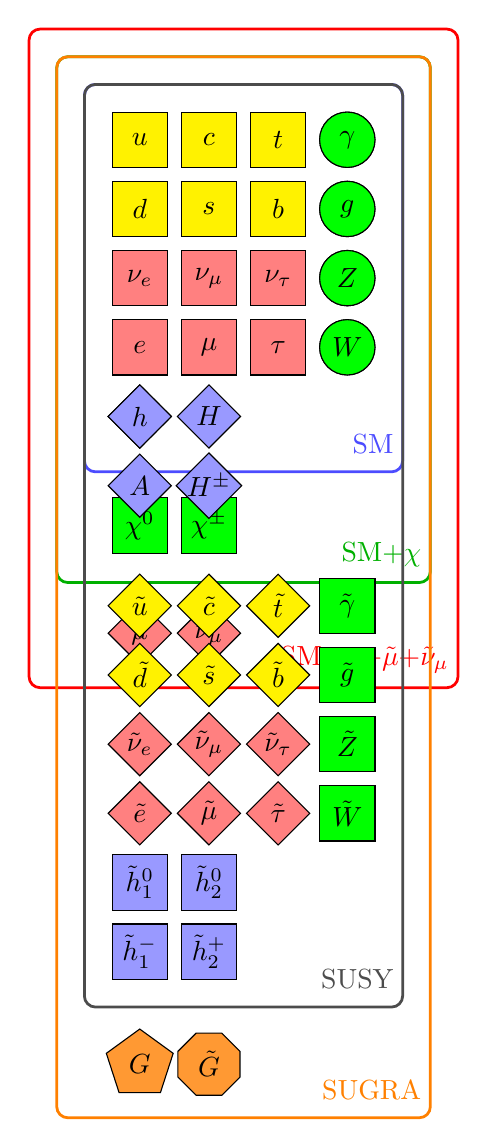
\begin{tikzpicture}[node distance = 2.5em, auto]
      \visible<1-4>{
      \node[quark] (u) {$u$};
      \node[quark, below of=u] (d) {$d$};
      \node[quark, right of=u] (c) {$c$};
      \node[quark, below of=c] (s) {$s$};
      \node[quark, right of=c] (t) {$t$};
      \node[quark, below of=t] (b) {$b$};
      \node[lepton, below of=d] (ne) {$\nu_e$};
      \node[lepton, below of=ne] (e) {$e$};
      \node[lepton, right of=ne] (nm) {$\nu_\mu$};
      \node[lepton, below of=nm] (m) {$\mu$};
      \node[lepton, right of=nm] (nt) {$\nu_\tau$};
      \node[lepton, below of=nt] (ta) {$\tau$};
      \node[gauge, right of=t] (gamma) {$\gamma$};
      \node[gauge, below of=gamma] (g) {$g$};
      \node[gauge, below of=g] (Z) {$Z$};
      \node[gauge, below of=Z] (W) {$W$};
      \node[phantom, below of=W] (corner) {\phantom{X}};
      \node[phantom, below of=corner] (corner2) {\phantom{X}};
      \draw[line width=1, color=blue!70,rounded corners] ($(u) + (-2em,2em)$) rectangle ($(corner) + (2em,-2em)$);
      \node[color=blue!70, anchor=east] (MSSM) at ($(corner.east) + (1em,-1em)$) {SM};
      }
      \visible<1>{
        \node[scalar, fill=blue!10, dashed, below of=e] (h) {$h$};
      }
      \visible<2-4>{
        \node[scalar, below of=e] (h) {$h$};
      }
      \visible<3-4>{
        \node[gaugino, below=1.75em of h] (chi0) {$\chi^{0}$};
        \node[gaugino, right of=chi0] (chipm) {$\chi^{\pm}$};
        \draw[line width=1, color=darkgreen,rounded corners] ($(u) + (-3em,3em)$) rectangle ($(corner2) + (3em,-3.5em)$);
        \node[color=darkgreen, anchor=east] (Split) at ($(corner2.east) + (2em,-2.5em)$) {SM+$\chi$};
      }
      \visible<4>{
        \node[slepton, below=1.7em of chi0] (smu) {$\tilde\mu$};
        \node[slepton, right of=smu] (snu) {$\tilde{\nu}_{\mu}$};
        \draw[line width=1, color=red,rounded corners] ($(u) + (-4em,4em)$) rectangle ($(corner2) + (4em,-7.3em)$);
        \node[color=red, anchor=east] (Split) at ($(corner2.east) + (3em,-6.3em)$) {SM+$\chi$+$\tilde{\mu}$+$\tilde{\nu}_\mu$};
      }
      \visible<5->{
        \node[quark] (u) {$u$};
        \node[quark, below of=u] (d) {$d$};
        \node[quark, right of=u] (c) {$c$};
        \node[quark, below of=c] (s) {$s$};
        \node[quark, right of=c] (t) {$t$};
        \node[quark, below of=t] (b) {$b$};
        \node[lepton, below of=d] (ne) {$\nu_e$};
        \node[lepton, below of=ne] (e) {$e$};
        \node[lepton, right of=ne] (nm) {$\nu_\mu$};
        \node[lepton, below of=nm] (m) {$\mu$};
        \node[lepton, right of=nm] (nt) {$\nu_\tau$};
        \node[lepton, below of=nt] (ta) {$\tau$};
        \node[gauge, right of=t] (gamma) {$\gamma$};
        \node[gauge, below of=gamma] (g) {$g$};
        \node[gauge, below of=g] (Z) {$Z$};
        \node[gauge, below of=Z] (W) {$W$};
        \node[scalar, below of=e] (h) {$h$};
        \node[scalar, right of=h] (H) {$H$};
        \node[scalar, below of=h] (A) {$A$};
        \node[scalar, right of=A] (Hpm) {$H^\pm$};
        %
        \node[squark, below=2em of A] (su) {$\tilde u$};
        \node[squark, below of=su] (sd) {$\tilde d$};
        \node[squark, right of=su] (sc) {$\tilde c$};
        \node[squark, below of=sc] (ss) {$\tilde s$};
        \node[squark, right of=sc] (st) {$\tilde t$};
        \node[squark, below of=st] (sb) {$\tilde b$};
        \node[slepton, below of=sd] (sne) {$\tilde \nu_e$};
        \node[slepton, below of=sne] (se) {$\tilde e$};
        \node[slepton, right of=sne] (snm) {$\tilde \nu_\mu$};
        \node[slepton, below of=snm] (sm) {$\tilde \mu$};
        \node[slepton, right of=snm] (snt) {$\tilde \nu_\tau$};
        \node[slepton, below of=snt] (sta) {$\tilde \tau$};
        \node[gaugino, right of=st] (sgamma) {$\tilde \gamma$};
        \node[gaugino, below of=sgamma] (sg) {$\tilde g$};
        \node[gaugino, below of=sg] (sZ) {$\tilde Z$};
        \node[gaugino, below of=sZ] (sW) {$\tilde W$};
        \node[higgsino, below of=se] (sh) {$\tilde h_1^0$};
        \node[higgsino, right of=sh] (sH) {$\tilde h_2^0$};
        \node[higgsino, below of=sh] (sA) {$\tilde h^-_1$};
        \node[higgsino, below of=sH] (sHpm) {$\tilde h^+_2$};
        \node[phantom, below of=sW    ] (sZprime) {\phantom{X}};
        \node[phantom, below of=sZprime] (corner) {\phantom{X}};
        \node[phantom, below of=corner] (corner2) {\phantom{X}};
        %
        \draw[line width=1, color=black!70,rounded corners] ($(u) + (-2em,2em)$) rectangle ($(corner) + (2em,-2em)$);
        \node[color=black!70, anchor=east] (SUSY) at ($(corner.east) + (1em,-1em)$) {SUSY};
      }
      \visible<6->{
        \node[graviton, below=1.75em of sA] (G) {$G$};
        \node[gravitino, right of=G] (sG) {$\tilde{G}$};
        \draw[line width=1, color=orange, rounded corners] ($(u) + (-3em,3em)$) rectangle ($(corner2) + (3em,-3.5em)$);
        \node[color=orange, anchor=east] (SUGRA) at ($(corner2.east) + (2em,-2.5em)$) {SUGRA};
      }
    \end{tikzpicture}}
    \column{.7\linewidth}
    \emph{Open questions:}\\
    \begin{itemize}
    \item {\color<2->{darkgreen}{Does the Higgs exist?}}
    \item {\color<3->{darkgreen}{What does DM consist of?}}
    \item {\color<4->{darkgreen}{What causes the deviation of $(g-2)_\mu$?}}
    \item {\color<5->{darkgreen}{Is the vacuum stable up to $M_{\text{Pl}}$?}}
    \item {\color<5->{darkgreen}{Why is $M_h = 125\eh{GeV}$?}}
    \item {\color<5->{darkgreen}{Is there a solution to the hierarchy problem?}}
    \item {\color<6->{darkgreen}{Can QFT and gravity be unified?}}
    \end{itemize}
  \end{columns}
\end{frame}

%%%%%%%%%%%%%%%%%%%%%%%%%%%%%%%%%%%%%%%%

\begin{frame}{Many extensions of the Standard Modell must be studied}
  \begin{center}
    \includegraphics[width=\textwidth]{images/FS.png}
  \end{center}
  \onslide<2>{%
  \tikz[overlay,remember picture] 
  \node[at=(current page.north east),anchor=north east,inner sep=0pt, xshift=-1.5cm, yshift=-2cm] (FS) {
    \textbf{FlexibleSUSY}};
  \tikz[overlay,remember picture] 
  \draw[-latex,thick] ([yshift=-0.2cm] FS.south) to[out=270,in=0] ++(-2cm,-2cm);
}
\end{frame}

%%%%%%%%%%%%%%%%%%%%%%%%%%%%%%%%%%%%%%%%

% \begin{frame}{Introduction}
%   Current status:
%   \begin{itemize}
%   \item SM is complete
%   \item no BSM particles found at the LHC so far
%   \end{itemize}
%   Currently open challenges:
%   \begin{itemize}
%   \item hierarchy problem
%   \item $\approx 3.6\sigma$ deviation between $g_\mu^\text{exp}$ und $g_\mu^\text{theo}$
%   \item Dark Matter, Dark Energy
%   \item unified description of all interactions, including gravity
%   \end{itemize}
%   Possible solutions:
%   \begin{itemize}
%   \item BSM physics (supersymmetry, \ldots)
%   \end{itemize}
% \end{frame}

%%%%%%%%%%%%%%%%%%%%%%%%%%%%%%%%%%%%%%%%

% \begin{frame}{SUSY particle exclusion limits}
%   \begin{center}
%     \includegraphics[width=\textwidth]{images/ATLAS_SUSY_Summary}
%   \end{center}
% \end{frame}

%%%%%%%%%%%%%%%%%%%%%%%%%%%%%%%%%%%%%%%%

\section{BSM Phenomenology with FlexibleSUSY}

\begin{frame}{Contents}
  \tableofcontents[currentsection]  
\end{frame}

\begin{frame}{What is FlexibleSUSY?}
  \begin{center}
    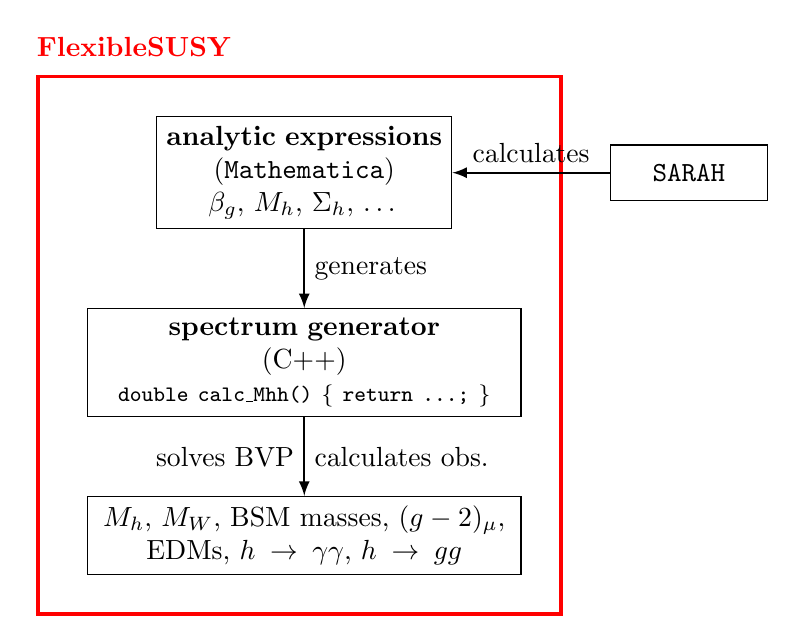
\begin{tikzpicture}
    \node[block] (EXPR) {\textbf{analytic expressions}\\ (\Mathematica)\\ $\beta_g$, $M_h$, $\Sigma_h$, \ldots};
    % \node[block, below = 1cm of EXPR, text width=15em] (FS) {\textbf{spectrum generator}\\ (C++)\\ solves BVP, calculates observables};
    \node[block, below = 1cm of EXPR, text width=15em] (FS) {\textbf{spectrum generator}\\ (C++)\\ \footnotesize{\texttt{double calc\_Mhh() \{ return ...; \}}}};
    \node[block, below = 1cm of FS, text width=15em] (OUT) {$M_h$, $M_W$, BSM masses, $(g-2)_\mu$, EDMs, $h\rightarrow\gamma\gamma$, $h\rightarrow gg$};
    \path[arrow] (EXPR) -- node[right]{generates} (FS);
    \path[arrow] (FS) -- node[right]{calculates obs.} node[left]{solves BVP} (OUT);
    \draw[red,very thick] ($(EXPR.north west)+(-1.5,0.5)$) node(FSname){} rectangle ($(OUT.south east)+(0.5,-0.5)$);
    \node[above right = 0cm and 0cm of FSname.north west] {\textbf{\textcolor{red}{FlexibleSUSY}}};
    \node[block, right = 2cm of EXPR, text width=5em] (SARAH) {\textbf{\SARAH}};
    \path[arrow] (SARAH) -- node[above]{calculates} (EXPR);
    \end{tikzpicture}
  \end{center}
\end{frame}

%%%%%%%%%%%%%%%%%%%%%%%%%%%%%%%%%%%%%%%%

\begin{frame}{Spectrum generator setup in FlexibleSUSY}
  \begin{raggedright}
    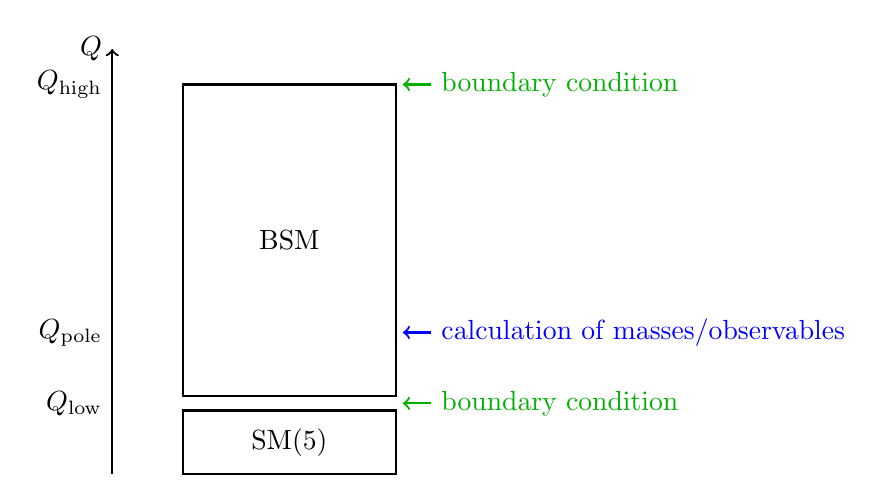
\begin{tikzpicture}[scale=0.9]
      \draw[->, thick] (0,0) -- (0,1) node[left]{$Q_\text{low}$} -- (0,2) node[left]{$Q_\text{pole}$} -- (0,5.5) node[left]{$Q_\text{high}$} -- (0,6) node[left] {$Q$};
      \draw[thick] (1,0)   rectangle node{SM(5)} (4,0.9);
      \draw[thick] (1,1.1) rectangle node{BSM} (4,5.5);
      \draw[<-, thick, darkgreen] (4.1,5.5) -- (4.5,5.5) node[right]{boundary condition};
      \draw[<-, thick, blue] (4.1,2) -- (4.5,2) node[right]{calculation of masses/observables};
      \draw[<-, thick, darkgreen] (4.1,1) -- (4.5,1) node[right]{boundary condition};
    \end{tikzpicture}
  \end{raggedright}
\end{frame}

%%%%%%%%%%%%%%%%%%%%%%%%%%%%%%%%%%%%%%%%

\begin{frame}{Example spectrum generator: MSSM}
  \begin{raggedright}
    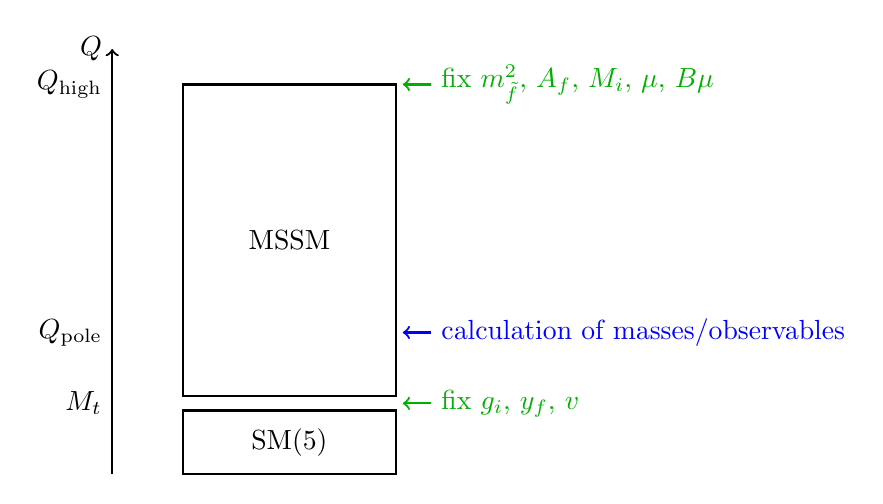
\begin{tikzpicture}[scale=0.9]
      \draw[->, thick] (0,0) -- (0,1) node[left]{$M_t$} -- (0,2) node[left]{$Q_\text{pole}$} -- (0,5.5) node[left]{$Q_\text{high}$} -- (0,6) node[left] {$Q$};
      \draw[thick] (1,0)   rectangle node{SM(5)} (4,0.9);
      \draw[thick] (1,1.1) rectangle node{MSSM} (4,5.5);
      \draw[<-, thick, darkgreen] (4.1,5.5) -- (4.5,5.5) node[right]{fix $m_{\tilde{f}}^2$, $A_f$, $M_i$, $\mu$, $B\mu$};
      \draw[<-, thick, blue] (4.1,2) -- (4.5,2) node[right]{calculation of masses/observables};
      \draw[<-, thick, darkgreen] (4.1,1) -- (4.5,1) node[right]{fix $g_i$, $y_f$, $v$};
    \end{tikzpicture}
  \end{raggedright}
\end{frame}

%%%%%%%%%%%%%%%%%%%%%%%%%%%%%%%%%%%%%%%%

\newenvironment{obsblock}[1]{%
  \setbeamercolor{block body}{bg=darkgreen!10}
  \setbeamercolor{block title}{bg=darkgreen}
  \begin{block}{#1}}{\end{block}}

\newenvironment{precblock}[1]{%
  \setbeamercolor{block body}{bg=darkred!10}
  \setbeamercolor{block title}{bg=darkred}
  \begin{block}{#1}}{\end{block}}

\newenvironment{flexblock}[1]{%
  \setbeamercolor{block body}{bg=blue!10}
  \setbeamercolor{block title}{bg=blue}
  \begin{block}{#1}}{\end{block}}

\newenvironment{speedblock}[1]{%
  \setbeamercolor{block body}{bg=black!10}
  \setbeamercolor{block title}{bg=black}
  \begin{block}{#1}}{\end{block}}

\begin{frame}{Features for all models (SUSY and non-SUSY)}
  \begin{columns}[T]
    \begin{column}{0.49\textwidth}
      \begin{obsblock}{Observables}
        $M_h$, $M_W$, BSM masses, $(g-2)_\mu$, EDMs,\\
        $h\rightarrow\gamma\gamma$, $h\rightarrow gg$
      \end{obsblock}
      \begin{flexblock}{Flexibility}
        multipe BVP solvers, user-defined BCs,\\ modular C++ code, \\
        SLHA input/output, \Mathematica\ input/output, SQLite output
      \end{flexblock}
    \end{column}
    \begin{column}{0.49\textwidth}
      \begin{precblock}{High precision}
        2L RGEs + 1L self energies (via \SARAH) + 1L thresholds,\\
        NLL resummation for $M_h$ (\texttt{FlexibleEFTHiggs})
      \end{precblock}
      \begin{speedblock}{High speed}
        multi-threading,\\ smart linear algebra,\\ lazy evaluation
      \end{speedblock}
    \end{column}
  \end{columns}
\end{frame}

%%%%%%%%%%%%%%%%%%%%%%%%%%%%%%%%%%%%%%%%

\newenvironment{modelblock}[1]{%
  \setbeamercolor{block body}{bg=darkyellow!15}
  \setbeamercolor{block title}{fg=black,bg=darkyellow}
  \begin{block}{#1}}{\end{block}}

\begin{frame}{Additional model-specific precision corrections}
  \begin{columns}[T]
    \begin{column}{0.49\textwidth}
      \begin{modelblock}{MSSM}
        3L RGEs, 3L $M_h$, 2L $M_{H,A,H^\pm}$, 2L $(g-2)_\mu$, 2L
        thresholds
      \end{modelblock}
      \begin{modelblock}{NMSSM}
        2L $M_h$, 2L $M_{H,A,H^\pm}$, 2L thresholds
      \end{modelblock}
      \begin{modelblock}{Split-MSSM}
        3L $M_h$, 2L thresholds for $y_t$, 2L thresholds for $\lambda$, $\tilde{g}_{ip}$
        the MSSM
      \end{modelblock}
    \end{column}
    \begin{column}{0.49\textwidth}
      \begin{modelblock}{SM}
        3L RGEs, 3L $M_h$, 3L thresholds for $\as$, $y_{t,b}$, 2L
        thresholds for $\lambda$ to the MSSM (\texttt{HSSUSY})
      \end{modelblock}
      \begin{modelblock}{THDM-II}
        2L thresholds for $\lambda_i$ to the MSSM
      \end{modelblock}
      \begin{modelblock}{THDM-II + $\tilde{h}$ + $\tilde{g}$}
        1L thresholds for $\lambda_i$ to the MSSM
      \end{modelblock}
    \end{column}
  \end{columns}
\end{frame}

%%%%%%%%%%%%%%%%%%%%%%%%%%%%%%%%%%%%%%%%

\section{Higgs Mass Calculations with FlexibleSUSY}

\begin{frame}{Contents}
  \tableofcontents[currentsection]  
\end{frame}

\begin{frame}{Interesting BSM physics: Supersymmetry}
  \emph{Properties:}
  \begin{itemize}
  \item gauge coupling unification
  \item can correctly predict $(g-2)_\mu$
  \item may contain a DM candidate $\chi_0$
  \item may solve the hierarchy problem
  \item ``predicts'' the Higgs boson mass
  \end{itemize}
  % \emph{Problems:}
  % \begin{itemize}
  % \item predicted Higgs mass too small?
  % \item no SUSY particles found so far
  % \end{itemize}
\end{frame}

% \begin{frame}{Interesting BSM physics: Supersymmetry}
%   \begin{columns}
%     \column{0.5\textwidth}
%     \emph{Properties:}
%     \begin{itemize}
%     \item {\color<1>{darkgreen}{gauge coupling unification}}
%     \item {\color<2>{darkgreen}{correct prediction of $(g-2)_\mu$}}
%     \item {\color<3>{darkgreen}{contains DM candidate}}
%     \item {\color<4>{darkgreen}{prediction of Higgs boson mass}}
%     \item {\color<5>{darkgreen}{solves the hierarchy problem}}
%     \end{itemize}
%     \emph{Problems:}
%     \begin{itemize}
%     \item predicted Higgs mass too small?
%     \item no SUSY particles found so far?
%     \end{itemize}
%     \column{0.5\textwidth}
%     \visible<1>{
%       \tikz[overlay,remember picture]
%       \node[anchor=center] at ($(current page.center)+(+3,0)$) {
%         \includegraphics[scale=0.5]{images/MSSM_gauge_couplings_largeMX}
%       };
%     }
%     \visible<2>{
%       \tikz[overlay,remember picture]
%       \node[anchor=center] at ($(current page.center)+(+3,0)$) {
%         \includegraphics[scale=0.5]{images/amu_SUSY}
%       };
%     }
%     \visible<3>{
%       \tikz[overlay,remember picture]
%       \node[anchor=center] at ($(current page.center)+(+3,0)$) {
%         \scalebox{3}{$\chi^0$}
%       };
%     }
%     \visible<4>{
%       \tikz[overlay,remember picture]
%       \node[anchor=center] at ($(current page.center)+(+3,0)$) {
%         \scalebox{2}{$m_h \le m_Z$}
%       };
%     }
%   \end{columns}
% \end{frame}

\begin{frame}{Prediction of the Higgs boson mass}
  \emph{SM:} (ad-hoc) Higgs potential:
  \begin{align*}
    V(\phi) &= \frac{\textcolor{red}{\lambda}}{8}\phi^4 - \frac{\mu^2}{2} \phi^2
    \intertext{$\Rightarrow$}
    m_h^2 &= \textcolor{red}{\lambda} v^2
    % \textcolor{darkgreen}{m_Z^2 = \frac{1}{4} \left(g_Y^2 + g_2^2\right) v^2}
  \end{align*}
  \emph{MSSM:} (required) Higgs potential:
  \begin{align*}
    V(\phi) &= \frac{1}{8}\textcolor{red}{\frac{1}{4}\left(g_Y^2 + g_2^2\right) \cos^2(2\beta)} \phi^4 + \cdots
    \intertext{$\Rightarrow$}
    m_h^2 &= \textcolor{red}{\frac{1}{4}\left(g_Y^2 + g_2^2\right) \cos^2(2\beta)} v^2 \\
    &= m_Z^2 \cos^2(2\beta) \\
    &\le m_Z^2
  \end{align*}
\end{frame}

\begin{frame}{Problem 1: no SUSY particles observed}
  \begin{center}
    \includegraphics[width=\textwidth]{images/ATLAS_SUSY_Summary}
  \end{center}
\end{frame}

\begin{frame}{Problem 2: Tree-level Higgs mass too small}
  (minimal) SUSY \emph{predicts} at tree-level:
  \begin{align*}
    m_h = m_Z |\cos 2\beta| \le m_Z
  \end{align*}
  But from experiment we know:
  \begin{align*}
    M_h &\approx 125.09 \GeV \\
    M_Z &\approx 91.2 \GeV
  \end{align*}
  $\Rightarrow$ \emph{large loop corrections} required!
  \begin{align*}
    M_h^2 &= m_h^2 + \Delta m_h^2
    & &\Rightarrow &
    \Delta m_h^2 &\geq (85\eh{GeV})^2
  \end{align*}
\end{frame}

% \begin{frame}{Eigenschaften des MSSM}
%   \begin{columns}
%     \column{0.5\textwidth}
%     \emph{Vorteile:}
%     \begin{itemize}
%     \item Eichkopplungsvereinigung
%     \item korrekte Vorhersage von $g_\mu$
%     \item Enthält ein Dunkle Materie-Teilchen
%     \item Vorhersage der Masse des Higgs-Bosons
%     \end{itemize}
%     \emph{Probleme:}
%     \begin{itemize}
%     \item {\color<1>{darkgreen}{vorhergesagte Higgs-Masse zu klein?}}
%     \item bisher keine SUSY-Teilchen gefunden?
%     \end{itemize}
%     \column{0.5\textwidth}
%   \end{columns}
%     \visible<1>{
%       \tikz[overlay,remember picture]
%       \node[anchor=center] at ($(current page.center)+(+3,0)$) {
%         \scalebox{2}{$m_h \le m_Z$}
%       };
%     }
% \end{frame}

% \begin{frame}{Problem: vorhergesagte Higgs-Masse zu klein?}
%   Vorhersage des MSSM:
%   \begin{align*}
%     % m_h^2 = m_Z^2 \cos^2(2\beta) \le m_Z^2
%     m_h \le m_Z
%   \end{align*}
%   Aus den Messungen am LEP und LHC wissen wir jedoch:
%   \begin{align*}
%     M_h &\approx 125.10 \GeV \\
%     M_Z &\approx 91.2 \GeV
%   \end{align*}
%   $\Rightarrow$ Das MSSM sagt nur dann die korrekte Higgs-Masse
%   vorher, wenn es \emph{große Quantenkorrekturen} zwischen $M_h$
%   und $m_h$ gibt!
%   \begin{align*}
%     M_h^2 &= m_h^2 + \Delta m_h^2
%     & &\Rightarrow &
%     \Delta m_h^2 &\geq (85\eh{GeV})^2
%   \end{align*}
% \end{frame}

% \begin{frame}{Eigenschaften des MSSM}
%   \begin{columns}
%     \column{0.5\textwidth}
%     \emph{Vorteile:}
%     \begin{itemize}
%     \item Eichkopplungsvereinigung
%     \item korrekte Vorhersage von $g_\mu$
%     \item Enthält ein Dunkle Materie-Teilchen
%     \item Vorhersage der Masse des Higgs-Bosons
%     \end{itemize}
%     \emph{Probleme:}
%     \begin{itemize}
%     \item vorhergesagte Higgs-Masse zu klein?
%       $\rightarrow$ Kein Problem!
%     \item {\color<1>{darkgreen}{bisher keine SUSY-Teilchen gefunden?}}
%     \end{itemize}
%     \column{0.5\textwidth}
%   \end{columns}
% \end{frame}

% \begin{frame}{Problem: bisher keine SUSY-Teilchen gefunden}
%   \begin{center}
%     \includegraphics[width=\textwidth]{images/ATLAS_SUSY_Summary}
%   \end{center}
% \end{frame}

\begin{frame}{How can we test a SUSY model?}
  \emph{Idea:}
  \begin{enumerate}
  \item Calculate $M_h$ as precisely as possible in the SUSY model:
  \begin{align*}
    M_h^2 &= m_h^2 + \Delta m_h^2
  \end{align*}
  \item Constrain the parameter space by requiring:
    \begin{align*}
      M_h \overset{!}{=} 125.09 \GeV \pm \Delta M_h^{\text{exp}} \pm \Delta M_h^{\text{theo}}
    \end{align*}
  \end{enumerate}
  \emph{Problem:} because of large loop corrections $\Delta m_h^2$:
  \begin{align*}
    \Delta M_h^{\text{theo}} &\gtrsim (1\ldots 2)\eh{GeV} \quad \text{at least!} \\
    \Delta M_h^{\text{exp}} &= 0.24\eh{GeV} \ \ \mycite{PDG-2017}
  \end{align*}
\end{frame}

%%%%%%%%%%%%%%%%%%%%%%%%%%%%%%%%%%%%%%%%%%%%%%%%%%%%%%%%%%%%

\begin{frame}{Contents}
  \tableofcontents[currentsection]
\end{frame}

%%%%%%%%%%%%%%%%%%%%%%%%%%%%%%%%%%%%%%%%%%%%%%%%%%%%%%%%%%%%

\begin{frame}{Approaches to predict $M_h$}
  \begin{center}
    \begin{tikzpicture}[scale=0.9]
      \draw[->, thick] (0,0) -- (0,1) node[left]{$M_t$} -- (0,5.5) node[left]{$\MS$} -- (0,6);
      \node at (2.5,7) {\emph{Fixed order}};
      \draw[thick] (1,0)   rectangle node{SM}    (4,0.9);
      \draw[thick] (1,1.1) rectangle node{MSSM}  (4,6);
      \draw[<-, thick, red] (4.1,5.5) -- (4.5,5.5) node[right]{$M_h$};
      \node at (7.5,7) {\emph{Effective Field Theory}};
      \draw[thick] (6,0)   rectangle node{SM}    (9,0.9);
      \draw[thick] (6,1.1) rectangle node{EFT}   (9,5.4);
      \draw[thick] (6,5.6) rectangle node{MSSM}  (9,6.5);
      \draw[<-, thick, red] (9.1,1.1) -- (9.5,1.1) node[right]{$M_h$};
    \end{tikzpicture}
  \end{center}
\end{frame}

% Argumentation:

% 1. classic approach: FO calculation -> large uncertainty due to
% heavy particles. -> discuss recent status (3-loop) and uncertainty

\subsection{Fixed-order}

\begin{frame}{Contents}
  \tableofcontents[currentsection,currentsubsection]
\end{frame}

\begin{frame}{Fixed-order calculation}
  \emph{Input:} $\aem(M_Z)$, $\as(M_Z)$, $G_F$, $M_Z$, $M_t$, $m_b(m_b)$, \ldots\\[2em]
  \begin{center}
    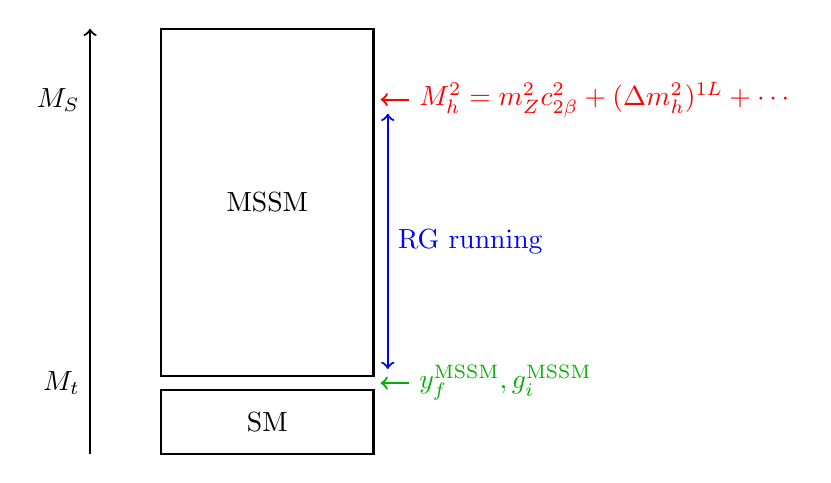
\begin{tikzpicture}[scale=0.9]
      \draw[->, thick] (0,0) -- (0,1) node[left]{$M_t$} -- (0,5) node[left]{$\MS$} -- (0,6);
      \draw[thick] (1,0)   rectangle node{SM}    (4,0.9);
      \draw[thick] (1,1.1) rectangle node{MSSM}  (4,6);
      \draw[<-, thick, red] (4.1,5) -- (4.5,5) node[right]{$M_h^2 = m_Z^2 c_{2\beta}^2 + (\Delta m_h^2)^{1L} + \cdots$};
      \draw[<-, thick, darkgreen] (4.1,1) -- (4.5,1) node[right]{$y_f^\MSSM, g_i^\MSSM$};
      \draw[<->, thick, blue] (4.2,1.2) -- node[right]{RG running} (4.2,4.8);
    \end{tikzpicture}
  \end{center}
\end{frame}

\begin{frame}{Fixed loop order calculation}
  Dominant contribution to $M_h$ at the 1-loop level:
  \begin{align*}
    (\Delta m_h^2)^{1L} &= -\Sigma_h^{1L}(p^2) + \frac{t_h^{1L}}{v} \\
    &= \fmfvcenter{htop} + \fmfvcenter{hstop} + \fmfvcenter{hstopA} \\
    &\phantom{={}} + \fmfvcenter{htoptad} + \fmfvcenter{hstoptad} \\
    &\approx \frac{12 m_t^2 y_t^2}{(4\pi)^2} \left(
      \ln\frac{\MS^2}{m_t^2}
      + \frac{X_t^2}{\MS^2}
      - \frac{X_t^4}{12 \MS^4}
    \right) + O(p^2)
  \end{align*}
\end{frame}

\begin{frame}{Higgs mass at 1-loop level}
  \begin{align*}
    (\Delta m_h^2)^{1L} &\approx
    \frac{12 m_t^2 y_t^2}{(4\pi)^2} \left(
      \ln\frac{\MS^2}{m_t^2}
      + \frac{X_t^2}{\MS^2}
      - \frac{X_t^4}{12 \MS^4}
    \right) + O(p^2)
  \end{align*}
  $X_t = A_t - \mu/t_\beta$ = stop mixing parameter,
  $\MS = (m_Q)_{33} = (m_U)_{33}$
  % 24 mt^4 / (16 Pi^2 v^2) (Log[MS^2/mt^2] + Xt^2/MS^2 - Xt^4/(12 MS^4))
  \\[1em]
  \emph{Observations:}
  \begin{itemize}
  \item logarithmically enhanced by $\MS / m_t$
  \item maximal for $X_t \approx \sqrt{6} \MS$
  \item high sensitivity on $m_t$, due to prefactor $m_t^2 y_t^2 = 2 m_t^4/v^2$
  \item ambiguity of definition of $m_t$: pole mass or \DRbar\ mass? \\
    $M_t \approx 173.3\eh{GeV}$, $m_t^{\DRbar} \approx 165\eh{GeV}$ \\
    $\Rightarrow$ huge theoretical uncertainty!\\
    $\Rightarrow$ 2-loop calculation needed to resolve this ambiguity
  \item $M_h \approx 125\eh{GeV}$ requires $\MS \gtrsim 5\eh{TeV}$
  \end{itemize}
\end{frame}

\begin{frame}{Higgs mass at 2-loop level}
  Known contributions: $O(\as (\at + \ab) + (\at+\ab)^2 + \atau^2)$
  for $p^2 = 0$ \mycite{hep-ph/0105096, hep-ph/0112177}
  \\[1em]
  \includegraphics[width=0.6\textwidth]{images/atas}\\[1em]
  \includegraphics[width=\textwidth]{images/atat}
\end{frame}

\begin{frame}{Higgs mass at 2-loop level}
  \begin{align*}
    (\Delta m_h^2)^{2L} &\approx
    \frac{m_t^2 y_t^4}{(4\pi)^4} \left(
      c_1 \ln^2\frac{\MS^2}{m_t^2}
      + c_2 \ln\frac{\MS^2}{m_t^2}
      + c_3
    \right) \\
    & +
    \frac{m_t^2 y_t^2 g_3^2}{(4\pi)^4} \left(
      c_4 \ln^2\frac{\MS^2}{m_t^2}
      + c_5 \ln\frac{\MS^2}{m_t^2}
      + c_6
    \right)
  \end{align*}
  \emph{Observations:}
  \begin{itemize}
  \item logarithmically enhanced by $\MS / m_t$
  \item still high sensitivity on $m_t$
  \item ambiguity of definition of $m_t$ is resolved \ok
  \item ambiguity of definition of $\as$: $\as^\SM(M_Z)$, $\as^\MSSM(\MS)$, \ldots ? \\
    $\Rightarrow$ 3-loop calculation needed to resolve this ambiguity
  \end{itemize}
\end{frame}

\begin{frame}{Higgs mass at 3-loop level}
  Known contributions: $O(\at\as^2)$ for $p^2 = 0$ \mycite{1005.5709,1708.05720}
  \begin{center}
    \includegraphics[width=0.9\textwidth]{images/h3l-atasas}
  \end{center}
  \begin{align*}
    (\Delta m_h^2)^{3L} &\approx
    \frac{m_t^2 y_t^2 g_3^4}{(4\pi)^6} \left(
      c_7 \ln^3\frac{\MS^2}{m_t^2}
      + c_8 \ln^2\frac{\MS^2}{m_t^2}
      + c_9 \ln\frac{\MS^2}{m_t^2}
      + c_{10}
    \right)
  \end{align*}
  \emph{Observations:}
  \begin{itemize}
  \item logarithmically enhanced by $\MS / m_t$
  \item still high sensitivity on $m_t$
  \item ambiguity of definition of $m_t$ is resolved \ok
  \item ambiguity of definition of $\as$ is resolved \ok
  \end{itemize}
\end{frame}

\begin{frame}{Summary of fixed loop order calculation}
  Typical order of magnitude of loop contributions (depends on
  parameter scenario):
  \begin{align*}
    M_h &= m_h + \Delta m_h^{1L} + \Delta m_h^{2L} + \Delta m_h^{3L} + \cdots \\
    &\approx [91 + O(20\ldots 30) + O(2\ldots 4) + O(1\ldots 2)] \eh{GeV}
  \end{align*}
  \emph{Advantages:}
  \begin{itemize}
  \item includes logarithmic, non-logarithmic and suppressed terms of
    $O(v^2/\MS^2)$ at fixed loop order
  \item precise prediction if $\MS \sim m_t$
  \end{itemize}
  \emph{Problem:}
  \begin{itemize}
  \item large logarithmic corrections if $\MS \gg m_t$ \\
    $\Rightarrow$ slow convergence of perturbation series \\
    $\Rightarrow$ large theoretical uncertainty, ($1$--$2\eh{GeV}$, or
    more)
    % \\
    % recall: $M_h^{\text{exp}} = (125.09 \pm 0.24)\eh{GeV}$
  \end{itemize}
  % \emph{Note:} 3-loop MSSM corrections available in \Himalaya \mycite{1708.05720}
\end{frame}

\begin{frame}{Uncertainty estimate of the fixed-order \DRbarp\ calculation}
  \begin{center}
    \includegraphics[width=0.49\textwidth]{{{plots/SOFTSUSY/SS_TB-20_Xt--sqrt6}}}\hfill
    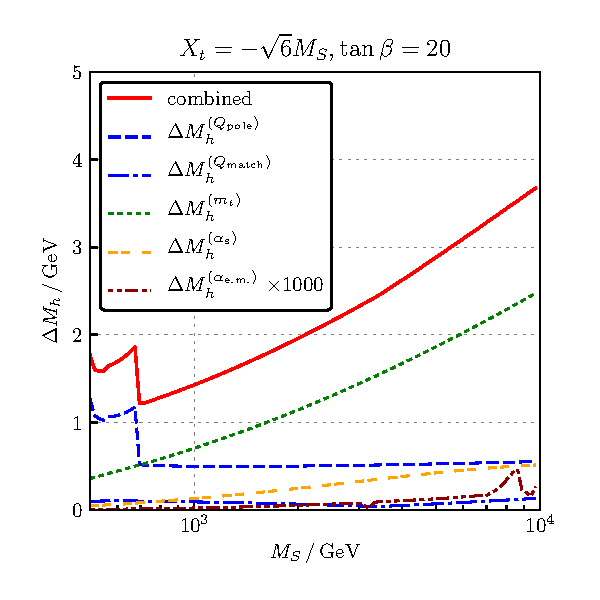
\includegraphics[width=0.49\textwidth]{{{plots/SOFTSUSY/SS_TB-20_Xt--sqrt6_individual}}}
  \end{center}
  \mycite{1804.09410}
\end{frame}

%%% EFT %%%%%%%%%%%%%%%%%%%%%%%%%%%%%%%%%%%%%%%%%%%%%%%

% colored SUSY particles are probably heavy -> this scenario is
% possibly most realistic

% 2. EFT approach: since colored SUSY particles are heavy -> construct
% different EFTs: SM, SM+split, 2HDM, 2HDM+split
%
% a) simplest option: SM-like:
% - pure EFT calculation is possible -> compare to FO!
% - hybrid approach is possible (Flexibleefthiggs or FH-approach)
%   (can be fully automatized due to its simplicity)
%
% b) advanced options: 2HDM-like
% -> show some plots with uncertainty est. from Bagnaschi/Weiglein/Voigt

% Conclusion: In the MSSM EFT calculation is most precise above ~ 1TeV
% Beyond MSSM: not so clear
% Flexibleefthiggs:  very precise and easy to automate
% UOLEA: only 1-loop, but incl. h.o. operators, easy to automate

%%%%%%%%%%%%%%%%%%%%%%%%%%%%%%%%%%%%%%%%

\subsection{Effective Field Theory}

\begin{frame}{Contents}
  \tableofcontents[currentsection,currentsubsection]
\end{frame}

\begin{frame}{Higgs mass calculation in an EFT}
  \emph{Idea:} Decouple SUSY particles at $\MS$ (expand in $v^2/\MS^2$) \\
  $\Rightarrow$ $\lambda(\MS)$ is fixed by the MSSM \\
  % $\Rightarrow$ effectively: separation of scales $\MS$ and $M_t$.
  \begin{center}
    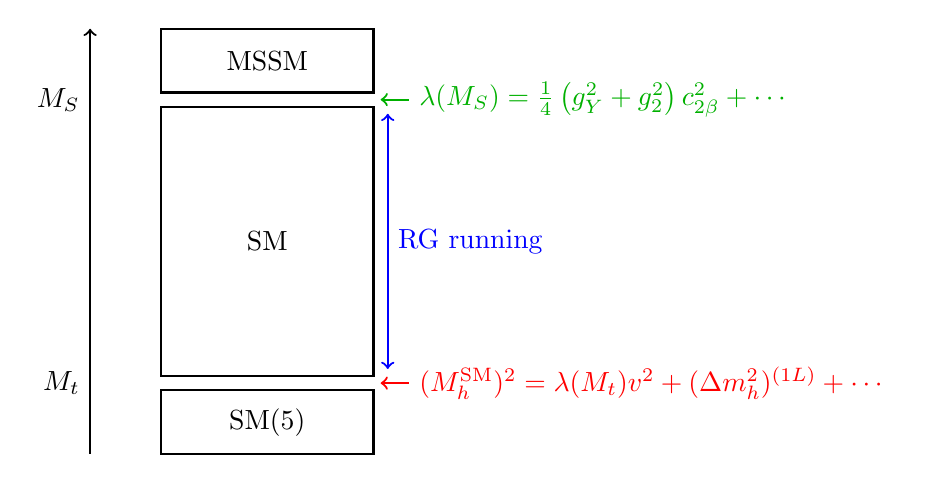
\begin{tikzpicture}[scale=0.9]
      \draw[->, thick] (0,0) -- (0,1) node[left]{$M_t$} -- (0,5) node[left]{$\MS$} -- (0,6);
      \draw[thick] (1,0)   rectangle node{SM(5)} (4,0.9);
      \draw[thick] (1,1.1) rectangle node{SM}    (4,4.9);
      \draw[thick] (1,5.1) rectangle node{MSSM}  (4,6);
      \draw[<-, thick, darkgreen] (4.1,5) -- (4.5,5) node[right]{$\lambda(\MS) = \frac{1}{4}\left(g_Y^{2} + g_2^2\right) c^2_{2\beta} + \cdots$};
      \draw[<-, thick, red] (4.1,1) -- (4.5,1) node[right]{$(M_h^\SM)^2 = \lambda(M_t) v^2 + (\Delta m_h^2)^{(1L)} + \cdots$};
      \draw[<->, thick, blue] (4.2,1.2) -- node[right]{RG running} (4.2,4.8);
    \end{tikzpicture}
  \end{center}
\end{frame}

% \begin{frame}{EFT avoids large logarithmic corrections}
%   \begin{enumerate}
%   \item Calculate $\lambda$ from the condition ($p^2 = v^2 = 0$):
%     \begin{align*}
%       \partial_{p^2}^{(k)}\Gamma_{h,\ldots,h}^{\MSSM,(n)}
%       = \partial_{p^2}^{(k)}\Gamma_{h,\ldots,h}^{\SM,(n)}
%     \end{align*}
%     $\Rightarrow$
%     \begin{align*}
%       \lambda(Q) &= \frac{1}{4}\left[g_Y^{2} + g_2^2\right] c^2_{2\beta}
%                    + \Delta \lambda^{1L} + \Delta \lambda^{2L} + \cdots \\
%                  &= \frac{1}{4}\left[g_Y^{2} + g_2^2\right] c^2_{2\beta}
%       + \frac{12 m_t^2 y_t^2}{(4\pi)^2 v^2} \left[
%         \ln\frac{\MS^2}{Q^2} + \frac{X_t^2}{\MS^2} - \frac{X_t^4}{12 \MS^4}
%       \right]
%       + \cdots
%     \end{align*}
%     $\Rightarrow$ \textcolor{darkgreen}{no large logs for $Q\approx\MS$}
%   \item RG running of $\lambda$ from $Q = \MS$ $\rightarrow M_t$.\\
%     $\Rightarrow$ \textcolor{darkgreen}{logs are resummed to all orders}
%   \item Calculate $M_h$ in the SM at $Q = M_t$:
%     \begin{align*}
%       (M_h^\SM)^2 &= \lambda(Q) v^2 + \frac{12 m_t^2 y_t^2}{(4\pi)^2 v^2} \ln\frac{Q^2}{m_t^2} + \cdots
%     \end{align*}
%     $\Rightarrow$ \textcolor{darkgreen}{no large logs for $Q\approx M_t$}
%   \end{enumerate}
% \end{frame}

\begin{frame}{Summary of EFT approach}
  Typical order of magnitude of loop contributions (depends on
  parameter scenario, here $X_t = 0$, $\MS = 20\eh{TeV}$):
  \begin{align*}
    M_h &= m_h + \Delta m_h^{1L} + \Delta m_h^{2L} + \Delta m_h^{3L} + \cdots \\
    % &= \sqrt{\lambda(M_t)} v + \Delta m_h^{1L} + \Delta m_h^{2L} + \cdots \\
    &\approx [O(124) + O(0.5\ldots 1) + O(0.1\ldots 0.2) + O(0.02\ldots 0.04)] \eh{GeV}
    % &= \sqrt{\lambda(\MS)} v + \text{logs} + \Delta m_h^{1L} + \Delta m_h^{2L} + \cdots \\
    % &\approx [O(84) + O(40) + O(0.5\ldots 1) + O(0.1\ldots 0.2)] \eh{GeV}
  \end{align*}
  \emph{Advantages:}
  \begin{itemize}
  \item large logarithmic fixed order loop corrections are avoided
  \item large logarithms $\propto\ln(M_S/M_t)$ are resummed to all orders
  \end{itemize}
  \emph{Disadvantage:} terms of $O(v^2/M_S^2)$ are neglected \\
  $\Rightarrow$ imprecise when $v \sim \MS$ \\
  $\Rightarrow$ large theoretical uncertainty when $v \sim \MS$
\end{frame}

\begin{frame}{Comparison of fixed-order and EFT calculation}
  \begin{center}
    \includegraphics[width=0.49\textwidth]{plots/SOFTSUSY/Mh_MS_TB-20_Xt--sqrt6}\hfill
    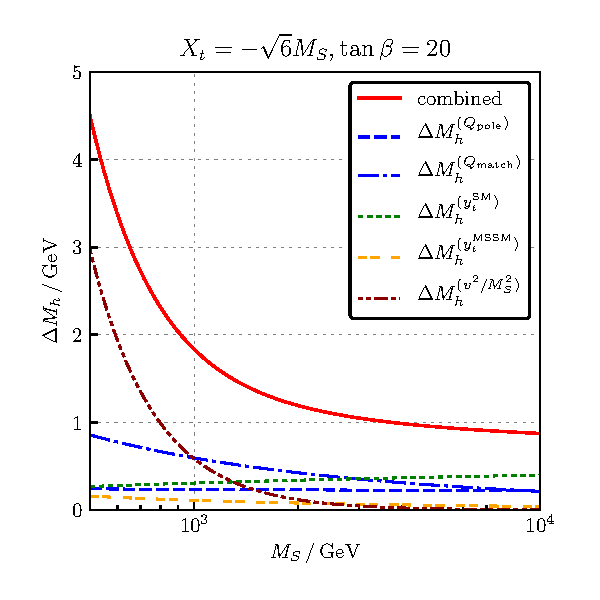
\includegraphics[width=0.49\textwidth]{plots/SOFTSUSY/HSSUSY_TB-20_Xt--sqrt6_individual}
  \end{center}
  \begin{center}
    $\DMh \overset{!}{=} \DMhHSSUSY$\\[0.5em]
    $\Rightarrow$ $\MS^{\text{equal}} = 1.0$--$1.3\TeV$ for
    small/large $\tan\beta$ and/or $X_t$
  \end{center}
  \mycite{1804.09410}
\end{frame}

\begin{frame}{Summary of fixed-order and EFT approaches}
  \begin{center}
    \begin{tabular}{lcc}
      \toprule
                  & low $\MS$ & high $\MS$ \\
                  & $\MS \lesssim 1\eh{TeV}$ & $\MS \gtrsim 1\eh{TeV}$ \\
      \midrule
      fixed-order & \ok       & \notok     \\
      EFT         & \notok    & \ok        \\
      ? hybrid    & \ok       & \ok        \\
      \bottomrule
    \end{tabular}
  \end{center}
  \vspace{2em}
  Q: Can the fixed-order and EFT approaches be combined? \\[1em]
  A: Yes!  \mycite{1312.4937, 1609.00371, 1710.03760, 1910.03595, 2003.04639}
\end{frame}

%%%%%%%%%%%%%%%%%%%%%%%%%%%%%%%%%%%%%%%%

\subsection{Hybrid}

\begin{frame}{Contents}
  \tableofcontents[currentsection,currentsubsection]  
\end{frame}

\begin{frame}{Hybrid calculation -- FeynHiggs approach}
  \emph{Goal:} resum large logarithms \emph{and} include suppressed
  $O(v^2/\MS^2)$ terms
  \\[2em]
  \emph{Idea I:} (``FeynHiggs approach'' \mycite{1312.4937, 1706.00346, 1805.00867, 1910.03595})\\
  Replace logs from fixed-order calculation by resummed logs:
  \begin{align*}
    M_h^2 = (M_h^2)_{\text{fixed-order}} - (M_h^2)_{\text{logs}} + (M_h^2)_{\text{resummed logs}}
  \end{align*}
  \emph{Pro:}
  \begin{itemize}
  \item[\ok] approach applicable to any BSM model
  \item[\ok] any EFT can be used
  \end{itemize}
  \emph{Contra:}
  \begin{itemize}
  \item[\notok] requires knowledge of fixed-order and EFT expressions
  \item[\notok] care must be taken to avoid double counting
  \end{itemize}
\end{frame}

\begin{frame}{FeynHiggs approach in FlexibleSUSY at 3-loop}
  \begin{center}
    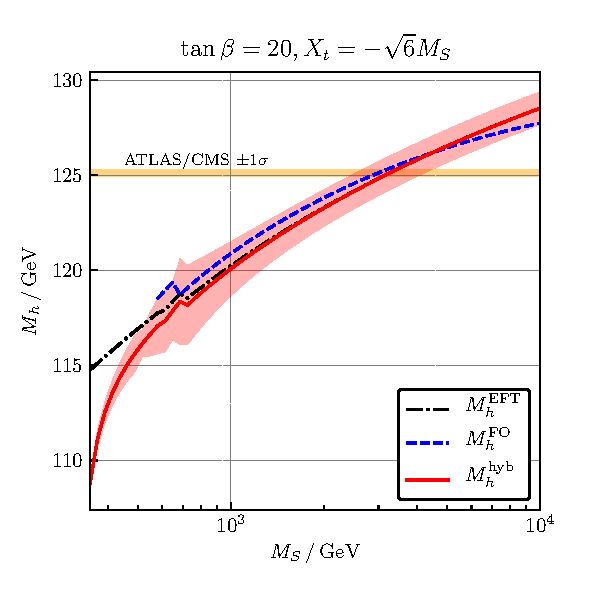
\includegraphics[width=0.49\textwidth]{plots/Mh3l-match-really/scan_Mh_MS_TB-20_Xt--sqrt6_mixed_3L}\hfill
    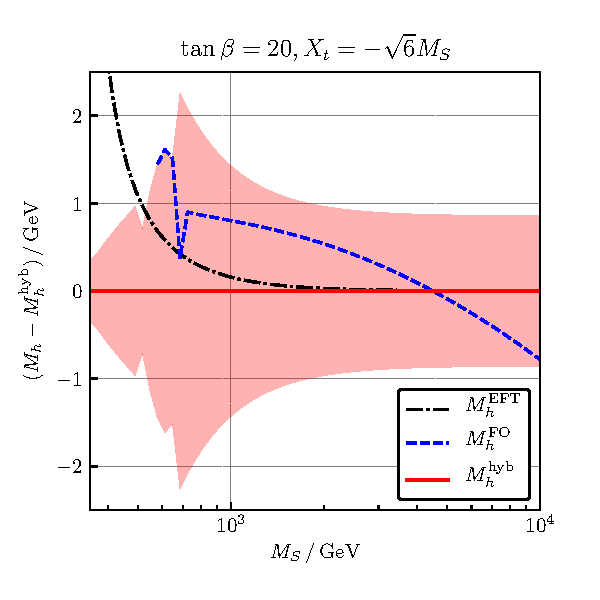
\includegraphics[width=0.49\textwidth]{plots/Mh3l-match-really/scan_Mh_MS_TB-20_Xt--sqrt6_mixed_3L_diff}
  \end{center}
  \mycite{1910.03595}
\end{frame}

\begin{frame}{Hybrid calculation -- FlexibleEFTHiggs}
  % \emph{Goal:} resum large logarithms \emph{and} include suppressed
  % $O(v^2/\MS^2)$ terms
  % \\[2em]
  \emph{Idea II:} (``FlexibleEFTHiggs'' \mycite{1609.00371,
    1710.03760, 2003.04639})\\
  Incorporate $O(v^2/\MS^2)$ terms into $\lambda$ by using the
  matching condition
  \begin{align*}
    (M_h^2)_{\SM} &\overset{!}{=} (M_h^2)_{\BSM} \qquad \text{at } Q = \MS \\
    \lambda(\MS) v^2 + (\Delta m_h^2)_{\SM} &= (M_h^2)_{\BSM}
  \end{align*}
  $\Rightarrow$
  \begin{align*}
    \lambda(\MS) = \frac{1}{v^2}\left[(M_h^2)_{\BSM} - (\Delta m_h^2)_{\SM}\right]
  \end{align*}
  Continue as in in the EFT calculation \ldots
  % \emph{Pro:}
  % \begin{itemize}
  % \item[\ok] approach applicable to any BSM model
  %   % easy to apply to any SM extensison
  % \item[\ok] easy to automate
  %   (only fixed-order expressions required)
  % \end{itemize}
  % \emph{Contra:}
  % \begin{itemize}
  % \item[\notok] difficult to extend to other EFTs beyond the SM (2HDM,
  %   \ldots)
  % \item[\meh] tricky to reach 2-loop accuracy\\
  %   (requires careful treatment of parameter matching)
  % \end{itemize}
\end{frame}

\begin{frame}{FlexibleEFTHiggs approach}
  Continue as in the EFT calculation:
  \begin{center}
    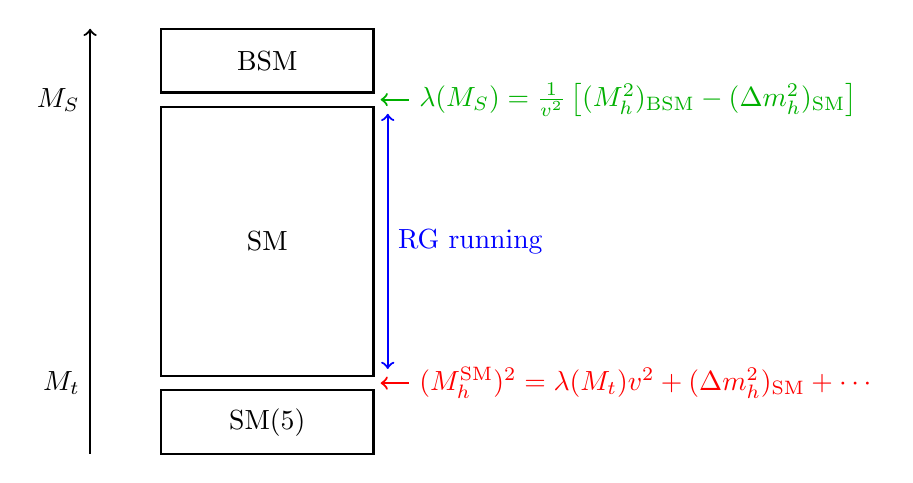
\begin{tikzpicture}[scale=0.9]
      \draw[->, thick] (0,0) -- (0,1) node[left]{$M_t$} -- (0,5) node[left]{$\MS$} -- (0,6);
      \draw[thick] (1,0)   rectangle node{SM(5)} (4,0.9);
      \draw[thick] (1,1.1) rectangle node{SM}    (4,4.9);
      \draw[thick] (1,5.1) rectangle node{BSM}  (4,6);
      \draw[<-, thick, darkgreen] (4.1,5) -- (4.5,5) node[right]{$\lambda(\MS) = \frac{1}{v^2}\left[(M_h^2)_{\BSM} - (\Delta m_h^2)_{\SM}\right]$};
      \draw[<-, thick, red] (4.1,1) -- (4.5,1) node[right]{$(M_h^\SM)^2 = \lambda(M_t) v^2 + (\Delta m_h^2)_{\SM} + \cdots$};
      \draw[<->, thick, blue] (4.2,1.2) -- node[right]{RG running} (4.2,4.8);
    \end{tikzpicture}
  \end{center}
\end{frame}

\begin{frame}{FlexibleEFTHiggs approach}
  Matching condition:
  \begin{align*}
    (M_h^2)_{\SM} &\overset{!}{=} (M_h^2)_{\BSM}
  \end{align*}
  \emph{Pro:}
  \begin{itemize}
  \item[\ok] approach applicable to any BSM model
    % easy to apply to any SM extensison
  \item[\ok] very simple $\rightarrow$ easy to automate
  \item[\ok] only BSM fixed-order expressions required
  \end{itemize}
  \emph{Contra:}
  \begin{itemize}
  \item[\notok] difficult to extend to other EFTs beyond the SM (2HDM,
    \ldots)
  \item[\meh] tricky to reach 2-loop accuracy\\
    (requires careful treatment of parameter matching)
  \end{itemize}
\end{frame}

\begin{frame}{Comparison of the three approaches in the MSSM}
  % Currently NLO + NLL is available \mycite{1609.00371, 1710.03760}.\\
  % Extension to NNLO + NNLL is work in progress:
  \begin{center}
    \includegraphics[width=0.49\textwidth]{{{plots/FlexibleEFTHiggs-2L/Mh_MS_TB-20_Xt-0}}}
    \hfill
    \includegraphics[width=0.49\textwidth]{{{plots/FlexibleEFTHiggs-2L/Mh_MS_TB-20_Xt--sqrt6}}}
  \end{center}
  in collaboration with Thomas Kwasnitza and Dominik Stöckinger
\end{frame}

\begin{frame}{FlexibleEFTHiggs approach}
  \begin{center}
    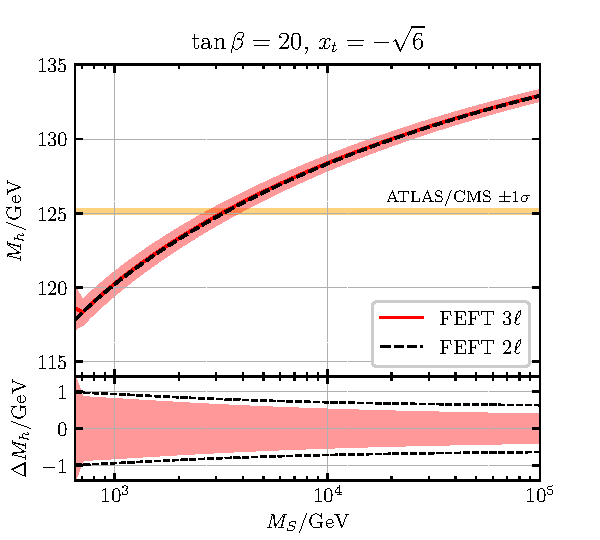
\includegraphics[width=0.49\textwidth]{{{plots/FlexibleEFTHiggs-3L/uncer_2panel_ms_scan_xt-sqrt6_tb20}}}\hfill
    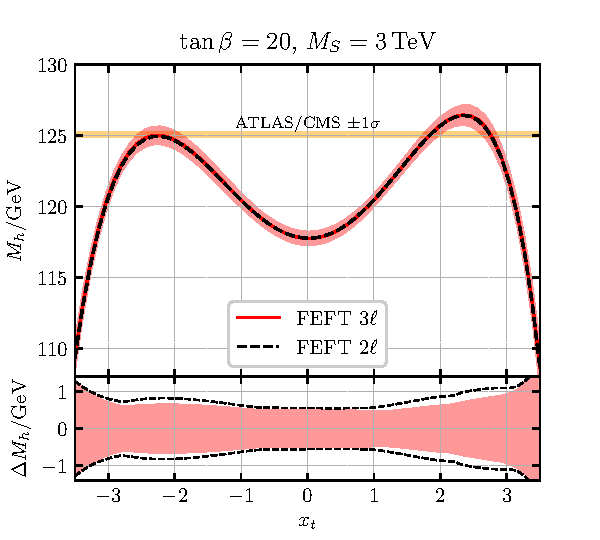
\includegraphics[width=0.49\textwidth]{{{plots/FlexibleEFTHiggs-3L/uncer_2panel_xt_scan_ms3_tb20}}}
  \end{center}
  \mycite{2003.04639}
\end{frame}

%%%%%%%%%%%%%%%%%%%%%%%%%%%%%%%%%%%%%%%%

\section{Summary}

%%%%%%%%%%%%%%%%%%%%%%%%%%%%%%%%%%%%%%%%

\begin{frame}{Berechnung bis zu endlicher Schleifenordnung}
  \begin{center}
    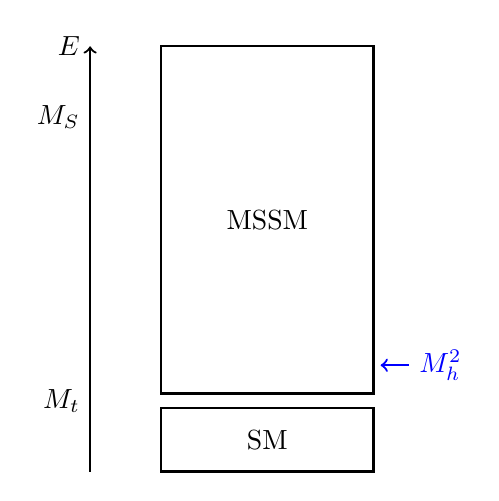
\begin{tikzpicture}[scale=0.9]
      \draw[->, thick] (0,0) -- (0,1) node[left]{$M_t$} -- (0,5) node[left]{$\MS$} -- (0,6) node[left] {$E$};
      \draw[thick] (1,0)   rectangle node{SM}    (4,0.9);
      \draw[thick] (1,1.1) rectangle node{MSSM}  (4,6);
      \draw[<-, thick, blue] (4.1,1.5) -- (4.5,1.5) node[right]{$M_h^2$};
      % \draw[<-, thick, darkgreen] (4.1,1) -- (4.5,1) node[right]{$y_f^\MSSM, g_i^\MSSM$};
      % \draw[<->, thick, blue] (4.2,1.2) -- node[right]{RG running} (4.2,4.8);
    \end{tikzpicture}
  \end{center}
\end{frame}

\begin{frame}{Berechnung bis zu endlicher Schleifenordnung}
  Quantenkorrekturen berechnen:
  \begin{align*}
    \Delta m_h^2 = \fmfvcenter{htop} + \fmfvcenter{hstop} + \fmfvcenter{hstop2} + \cdots
  \end{align*}
  \emph{Beobachtung:}
  \begin{itemize}
  \item Quantenkorrekturen lassen sich nach der Anzahl der Schleifen
    sortieren
  \item Jede Schleife ist proportional zu $\kappa = 1/(4\pi)^2 \approx 1/160$\\
    $\Rightarrow$ Feynman-Diagramm mit $n$ Schleifen ist proportional zu $\kappa^n$
  \item Je mehr Schleifen man mitnimmt, desto genauer das Ergebnis!
  \end{itemize}
  \vspace*{1em}
  \emph{Vorgehen:}
  Reihenentwicklung in Schleifen (Störungsreihe):
  \begin{align*}
    M_h^2 &= m_h^2 + \Delta m_h^2 \\
    \Delta m_h^2 &= \kappa^1 \Delta_1 + \kappa^2 \Delta_2 + \kappa^3 \Delta_3 + \cdots
  \end{align*}
\end{frame}

\begin{frame}{Los geht's! 1-Schleifen-Quantenkorrekturen}
  Quantenkorrekturen zu $M_h$ mit 1 Schleife:
  \begin{align*}
    \kappa^1\Delta_1
    &= \fmfvcenter{htop} + \fmfvcenter{hstop} + \cdots \\
    &\approx 6 \kappa y_t^4 v^2 \left(
      2L + c_0
    \right) + \cdots
  \end{align*}
  \\[1em]
  $L\equiv\ln(\MS / M_t)$ \\[0.5em]
  $M_t = 173.34\GeV$: Masse des Top-Quarks \\[0.5em]
  $\MS$: Masse der Stop-Quarks \\[0.5em]
  $c_0$ = konst.
  % $x_t \in [-4,4]$ = ``Strärke der Mischung der Stop-Quarks''
\end{frame}

\begin{frame}{1-Schleifen-Quantenkorrekturen}
  \begin{align*}
    \kappa^1\Delta_1
    &= \fmfvcenter{htop} + \fmfvcenter{hstop} + \cdots \\
    &\approx
    6 \kappa y_t^4 v^2 \left(
      2L + c_0
    \right) + \cdots
  \end{align*}
  % $X_t = A_t - \mu/t_\beta$ = stop mixing parameter,
  % $\MS = (m_Q)_{33} = (m_U)_{33}$
  % 24 mt^4 / (16 Pi^2 v^2) (Log[MS^2/mt^2] + Xt^2/MS^2 - Xt^4/(12 MS^4))
  \\[1em]
  \emph{Beobachtungen:}
  \begin{itemize}
  \item logarithmischer Beitrag mit $L\equiv\ln(\MS / M_t)$
  % \item maximal für $x_t \approx \sqrt{6}$
  % \item extrem sensitiv auf Wert von $y_t$
  \item damit Quantenkorrektur groß genug, so dass $M_h = 125.10\GeV$
    $\Rightarrow$ $\MS \gtrsim 2\TeV$
  \item verbleibende theoretische Unsicherheit: $\delta M_h^{\text{theo}} \approx \pm 6 \GeV$
  \end{itemize}
  \vspace*{1em}
  Nicht gut genug!
\end{frame}

\begin{frame}{Weiter geht's! 2-Schleifen-Quantenkorrekturen}
  \includegraphics[width=0.6\textwidth]{images/atas}\\[1em]
  \includegraphics[width=\textwidth]{images/atat}
  \\
  \vspace*{1em}
  \mycite{hep-ph/0105096, hep-ph/0112177}
\end{frame}

\begin{frame}{2-Schleifen-Quantenkorrekturen}
  \begin{align*}
    \kappa^2\Delta_2 &\approx
    \kappa^2 y_t^4 g_3^2 \left(
      c_1 L^2
      + c_2 L
      + c_3
    \right) + \cdots \\
  \end{align*}
  \emph{Beobachtungen:}
  \begin{itemize}
  \item logarithmischer Beitrag mit $L^2$, $L\equiv\ln(\MS / M_t)$
  % \item extrem sensitiv auf Wert von $y_t$
  \item verbleibende Unsicherheit: $\delta M_h^{\text{theo}} \approx \pm 3 \GeV$
  \end{itemize}
  \vspace*{1em}
  Immernoch nicht gut genug!
\end{frame}

\begin{frame}{Weiter geht's! 3-Schleifen-Quantenkorrekturen}
  \begin{center}
    \includegraphics[width=0.9\textwidth]{images/h3l-atasas}
  \end{center}
  \mycite{1005.5709}
  \begin{align*}
    \kappa^3\Delta_3 &\approx
    \kappa^3 y_t^4 g_3^4 \left(
      c_7 L^3
      + c_8 L^2
      + c_9 L
      + c_{10}
    \right)
  \end{align*}
  \emph{Beobachtungen:}
  \begin{itemize}
  \item logarithmischer Beitrag mit $L^3$, $L\equiv\ln(\MS / M_t)$
  % \item extrem sensitiv auf Wert von $y_t$
  \item verbleibende Unsicherheit: $\delta M_h^{\text{theo}} \approx \pm 2 \GeV$
  \end{itemize}
\end{frame}

\begin{frame}{Konvergenz der Störungsreihe}
  Typische Größenordnung der Quantenkorrekturen:
  \begin{align*}
    M_h &= m_h + \kappa^1\Delta_1 + \kappa^2\Delta_2 + \kappa^3\Delta_3 + \cdots \\
    &\approx [91 + O(20\ldots 30) + O(2\ldots 4) + O(1\ldots 2)] \GeV
  \end{align*}
  \emph{Beobachtung:}
  \begin{itemize}
  \item Störungsreihe konvergiert ``zu langsam''
  \end{itemize}
  \emph{Grund:}
  \begin{itemize}
  \item große Quantenkorrekturen sind nötig damit $M_h = 125.10\GeV$
  \item Quantenkorrektur mit $n$ Schleifen erzeugt Term $L^n$
  \item $\Rightarrow$ $L=\ln(\MS / M_t)$ muss groß gemacht werden!\\
    (möglich indem $\MS \gg M_t$, insbes.\ $\MS \gtrsim 2\TeV$)
  \item $\Rightarrow$ Störungsreihe konvergiert langsam
  % \item 4-Schleifen-Quantenkorrekturen aktuell nicht berechenbar
  \item $\Rightarrow$ verbleibende Unsicherheit durch Abschneiden der
    Störungsreihe: $\delta M_h^{\text{theo}} \approx 2\GeV$ \\
    zur Erinnerung: $\delta M_h^{\text{exp}} = 0.14\GeV$
  \end{itemize}
\end{frame}

\begin{frame}{Unsicherheitsabschätzung}
  \begin{center}
    \includegraphics[width=0.6\textwidth]{{{plots/SOFTSUSY/SS_TB-20_Xt--sqrt6}}}
  \end{center}
  \raggedleft\mycite{1804.09410}
\end{frame}

\begin{frame}{Lösung: Effektive Feldtheorie}
  \emph{Fazit:} Abschneiden der Störungsreihe auf 3-Schleifenniveau
  führt zu großen fehlenden Termen:
  \begin{align*}
    \Delta m_h^2\supset c_1 \kappa^1 L^1 + c_2 \kappa^2 L^2 + c_3 \kappa^3 L^3
    + O(\textcolor{red}{\kappa^4 L^4})
  \end{align*}
  \pause
  \emph{Lösung:} Verwende eine Methode, bei der \emph{alle} Terme von der Form
  \begin{align*}
    \Delta m_h^2 \supset \sum_{n=0}^\infty c_n \kappa^n L^n
  \end{align*}
  einbezogen werden:
  \begin{center}
    \emph{Effektive Feldtheorie (EFT)}
  \end{center}
\end{frame}

\begin{frame}{Contents}
  \tableofcontents[currentsection,currentsubsection]
\end{frame}

\begin{frame}{Feste Schleifenordnung vs.\ Effektive Feldtheorie}
  \begin{center}
    \begin{tikzpicture}[scale=0.9]
      \draw[->, thick] (0,0) -- (0,1) node[left]{$M_t$} -- (0,5) node[left]{$\MS$} -- (0,6) node[left] {$E$};
      \node at (2.5,7) {\emph{feste Schleifenordnung}};
      \draw[thick] (1,0)   rectangle node{SM}    (4,0.9);
      \draw[thick] (1,1.1) rectangle node{MSSM}  (4,6);
      \draw[<-, thick, blue] (4.1,1.5) -- (4.5,1.5) node[right]{$M_h$};
      \node at (7.5,7) {\emph{Effektive Feldtheorie}};
      \draw[thick] (6,0)   rectangle node{SM}   (9,4.9);
      \draw[thick] (6,5.1) rectangle node{MSSM}  (9,6);
      \draw[<-, thick, blue] (9.1,1.5) -- (9.5,1.5) node[right]{$M_h$};
    \end{tikzpicture}
  \end{center}
\end{frame}

\begin{frame}{Berechnung in einer Effektiven Feldtheorie}
  \emph{Idee:} SUSY-Teilchen entkoppeln an Energieskala $\MS$ \\
  $\Rightarrow$ SM ist ``Effektive Theorie'' (ohne SUSY-Teilchen)\\
  $\Rightarrow$ effektiver SM-Parameter $\lambda(\MS)$ wird vorhergesagt  \\
  % $\Rightarrow$ effectively: separation of scales $\MS$ and $M_t$.
  \begin{center}
    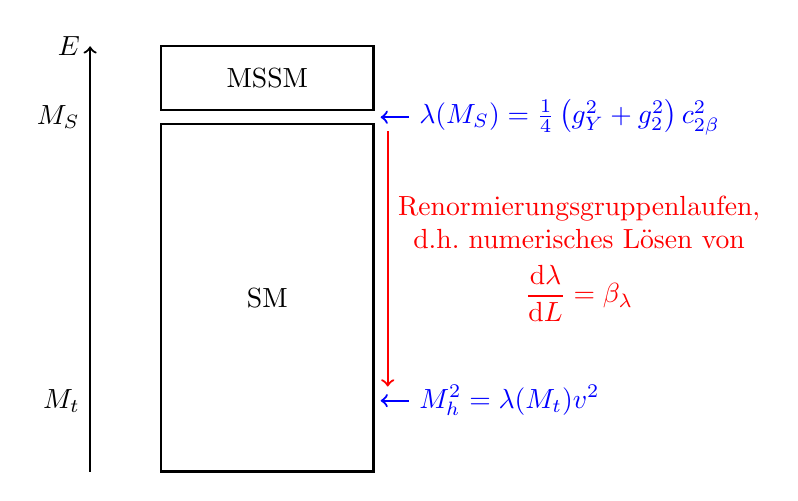
\begin{tikzpicture}[scale=0.9]
      \draw[->, thick] (0,0) -- (0,1) node[left]{$M_t$} -- (0,5) node[left]{$\MS$} -- (0,6) node[left] {$E$};
      \draw[thick] (1,0)   rectangle node{SM}    (4,4.9);
      \draw[thick] (1,5.1) rectangle node{MSSM}  (4,6);
      \draw[<-, thick, blue] (4.1,5) -- (4.5,5) node[right]{$\lambda(\MS) = \frac{1}{4}\left(g_Y^{2} + g_2^2\right) c^2_{2\beta}$};
      \draw[<-, thick, blue] (4.1,1) -- (4.5,1) node[right]{$M_h^2 = \lambda(M_t) v^2$};
      \draw[<-, thick, red] (4.2,1.2) -- node[right, align=center]{Renormierungsgruppenlaufen,\\
        d.h.\ numerisches Lösen von\\[0.5em]
        $\displaystyle\frac{\dd\lambda}{\dd L} = \beta_\lambda$} (4.2,4.8);
    \end{tikzpicture}
  \end{center}
\end{frame}

\begin{frame}{EFT enthält unendliche Reihe von $(\kappa L)^n$-Termen}
  System gekoppelter DGLs:
  \begin{align*}
    \frac{\dd\lambda}{\dd L} &= \beta_\lambda \approx -12 \kappa y_t^4 , &
    \frac{\dd y_t}{\dd L} &\approx -8 \kappa y_t g_3^2 , &
    \frac{\dd g_3}{\dd L} &\approx -7 \kappa g_3^3
  \end{align*}
  Lösung:
  \begin{align*}
    \lambda(M_t) &= \frac{1}{4}\left(g_Y^{2} + g_2^2\right) c^2_{2\beta} % \lambda(\MS)
                   - \frac{2 y_t^4}{3 g_3^2} \left[
                   \left( 1 + 14 g_3^2 \textcolor{red}{\kappa L} \right)^{-9/7} - 1
    \right]
  \end{align*}
  Einsetzen in $M_h^2 = \lambda(M_t) v^2$ ergibt:
  \begin{align*}
    M_h^2 &= m_Z^2 c^2_{2\beta}
            - \frac{2 y_t^4 v^2}{3 g_3^2} \left[
            \left( 1 + 14 g_3^2 \textcolor{red}{\kappa L} \right)^{-9/7} - 1
            \right]\\
          &= m_Z^2 c^2_{2\beta}
            + 12 y_t^4 v^2 \left[
            \textcolor{red}{\kappa L}
            - 16 g_3^2 \textcolor{red}{\kappa^2 L^2}
            + \frac{736}{3} g_3^4 \textcolor{red}{\kappa^3 L^3} + O(\textcolor{red}{\kappa^4L^4})
            \right]
  \end{align*}
  $\Rightarrow$ $M_h$ enthält \emph{unendliche Reihe} von $\textcolor{red}{(\kappa L)^n}$-Termen
\end{frame}

\begin{frame}{Eigenschaften der EFT-Rechnung}
  Typische Größenordnung der Quantenkorrekturen in einer EFT-Rechnung:
  \begin{align*}
    M_h &= m_h + \Delta m_h^{1\ell} + \Delta m_h^{2\ell} + \Delta m_h^{3\ell} + \cdots \\
    &\approx [O(124) + O(0.5\ldots 1) + O(0.1\ldots 0.2) + O(0.02\ldots 0.04)] \eh{GeV}
  \end{align*}
  \emph{Vorteile:}
  \begin{itemize}
  \item Störungsreihe wird nicht bei $n$ Schleifen $O(L^n)$
    abgeschnitten
  \item große Logarithmen $L^n$ werden komplett aufsummiert
  \item $\Rightarrow$ Störungsreihe konvergiert schnell
  \end{itemize}
  \vspace*{1em}
  \emph{Nachteil:}
  \begin{itemize}
  \item unpräzise wenn  $\MS \lesssim 0.5\TeV$
    (ist irrelevant)
  \end{itemize}
\end{frame}

\begin{frame}{Unsicherheitsabschätzung}
  \begin{center}
    \includegraphics[width=0.6\textwidth]{plots/SOFTSUSY/Mh_MS_TB-20_Xt--sqrt6}
  \end{center}
  \raggedleft\mycite{1804.09410}
\end{frame}

%%%%%%%%%%%%%%%%%%%%%%%%%%%%%%%%%%%%%%%%

\begin{frame}{Zusammenfassung}
  \emph{Supersymmetrie} ist eine interessante Erweiterung des
  Standardmodells.  Bietet Erklärungen für Dunkle Materie,
  $g_\mu$, uvm.
  \\[1em]
  \emph{Präzise Vorhersage der Masse des Higgs-Bosons} erlaubt
  Einschränkung des Parameterraums des MSSM.
  \\[1em]
  \emph{Stopmassen} $\MS \gtrsim 2\TeV$ im MSSM nötig für korrekte
  Vorhersage von $M_h = 125.10\GeV$ $\rightarrow$ Kompatible mit LHC-Ergebnissen.
  \\[1em]
  \emph{Effektive Feldtheorie} ist nötig um präzise Vorhersagen zu
  erhalten, da unendliche Reihe großer Logarithmen aufsummiert
\end{frame}

\begin{frame}{Ausblick}
  \begin{center}
    \LARGE Riesiger Zoo an SUSY-Modellen\\ $\Rightarrow$ Automatisierung nötig!
  \end{center}
  \begin{center}
    \includegraphics[width=0.9\textwidth]{images/FS.png}
  \end{center}
\end{frame}

%%%%%%%%%%%%%%%%%%%%%%%%%%%%%%%%%%%%%%%%
% backup slides
%%%%%%%%%%%%%%%%%%%%%%%%%%%%%%%%%%%%%%%%

\begin{frame}[noframenumbering]
  \begin{center}
    \Huge Backup
  \end{center}
\end{frame}

%%%%%%%%%%%%%%%%%%%%%%%%%%%%%%%%%%%%%%%%

\begin{frame}[noframenumbering]{Scenarios with 1 light Higgs doublet}
  \begin{center}
    \begin{tikzpicture}[scale=0.8, every node/.style={transform shape}]
      \draw[->, thick] (0,0) -- (0,1) node[left]{$M_t$} -- (0,4) node[left]{$\MS$} -- (0,6);
      \node at (2.5,7) {\emph{I high-scale SUSY}};
      \draw[thick] (1,0)   rectangle node{SM}    (4,0.9);
      \draw[thick] (1,1.1) rectangle node{SM}   (4,4.9);
      \draw[thick] (1,5.1) rectangle node{MSSM}  (4,6);
      % 
      \node at (6.5,7) {\emph{II split-SUSY}};
      \draw[thick] (5,0)   rectangle node{SM}    (8,1.9);
      \draw[thick] (5,2.1) rectangle node{SM + $\chi_i$ + $\tilde{g}$} (8,4.9);
      \draw[thick] (5,5.1) rectangle node{MSSM}  (8,6);
    \end{tikzpicture}
  \end{center}
\end{frame}

\begin{frame}[noframenumbering]{Scenarios with 2 light/intermediate Higgs doublets}
  \begin{center}
    \begin{tikzpicture}[scale=0.8, every node/.style={transform shape}]
      \draw[->, thick] (0,0) -- (0,1) node[left]{$M_t$} -- (0,4) node[left]{$\MS$} -- (0,6);
      \node[align=center] at (2.5,7) {\emph{III 2HDM}\\ (light $h_i$, $A$, $H^{\pm}$)};
      \draw[thick] (1,0)   rectangle node{SM} (4,0.9);
      \draw[thick] (1,1.1) rectangle node{2HDM} (4,4.9);
      \draw[thick] (1,5.1) rectangle node{MSSM} (4,6);
      % 
      \node[align=center] at (6.5,7) {\emph{IV 2HDM+split}\\ (light $h_i$, $A$, $H^{\pm}$,\\ intermediate $\chi_i$, $\tilde{g}$)};
      \draw[thick] (5,0)   rectangle node{SM} (8,0.9);
      \draw[thick] (5,1.1) rectangle node{2HDM} (8,2.9);
      \draw[thick] (5,3.1) rectangle node[align=center]{2HDM\\ + $\chi_i$ + $\tilde{g}$} (8,4.9);
      \draw[thick] (5,5.1) rectangle node{MSSM} (8,6);
      % 
      \node[align=center] at (10.5,7) {\emph{V 2HDM+split}\\ (light $\chi_i$, $\tilde{g}$, inter-\\ mediate $h_2$, $A$, $H^{\pm}$)};
      \draw[thick] (9,0)   rectangle node{SM} (12,0.9);
      \draw[thick] (9,1.1) rectangle node{SM + $\chi_i$ + $\tilde{g}$} (12,2.9);
      \draw[thick] (9,3.1) rectangle node[align=center]{2HDM\\ + $\chi_i$ + $\tilde{g}$} (12,4.9);
      \draw[thick] (9,5.1) rectangle node{MSSM} (12,6);
    \end{tikzpicture}
  \end{center}
\end{frame}

\end{document}
